\documentclass[11pt,letterpaper]{article}

\usepackage[T1]{fontenc}
\usepackage[utf8]{inputenc}
\usepackage{lmodern}
\usepackage[margin=1in]{geometry}
\usepackage{amsmath,amssymb}
\usepackage{booktabs}
\usepackage{tabularx}
\usepackage{graphicx}
\usepackage{float}
\usepackage[font=small,labelfont=bf]{caption}
\usepackage{subcaption}
\usepackage{enumitem}
\usepackage{microtype}
\usepackage{xcolor}
\usepackage[hidelinks]{hyperref}
\usepackage{url}
\usepackage{makecell}

\setlist{itemsep=2pt,topsep=4pt}
\setlength{\parskip}{4pt}
\renewcommand{\arraystretch}{1.12}
\newcommand{\cmark}{Yes}
\newcommand{\xmark}{No}

\title{\vspace{-0.6cm}\rule{\textwidth}{1.4pt}\\[10pt]
\textbf{VEYRA: A Digital Livestock Passport that Links Muzzle-Based Cattle Identification, Camera Health Monitoring, and an Approval-Gated AI Insurance Agent}\\[6pt]
\rule{\textwidth}{0.6pt}}

\newcommand{\authorbox}[4]{\begin{tabular}{c}\textbf{#1}\\ #2\\ #3\\ {\small\texttt{#4}}\end{tabular}}
\author{
\begin{tabular}{c@{\hspace{1.4cm}}c}
\authorbox{Athilla Zaidan Zidna Fann}{Informatics Engineering}{Institut Teknologi Bandung}{} &
\authorbox{Jason Edward Salim}{Informatics Engineering}{Institut Teknologi Bandung}{13524034@std.stei.itb.ac.id} \\ \noalign{\vskip 16pt}
\authorbox{Abel Gani}{Information Systems and Technology}{Institut Teknologi Bandung}{18224016@std.stei.itb.ac.id} &
\authorbox{Gregory William Sutjipto}{Information Systems and Technology}{Institut Teknologi Bandung}{18224010@std.stei.itb.ac.id} \\ \noalign{\vskip 16pt}
\multicolumn{2}{c}{\authorbox{Tiffany Viriya Chu}{Information Systems and Technology}{Institut Teknologi Bandung}{18224068@std.stei.itb.ac.id}}
\end{tabular}
}
\date{}

\begin{document}
\maketitle

\begin{abstract}
\noindent Cattle are the most valuable asset on a livestock farm, yet the records that protect them are scattered: identity lives on an ear tag, health observations in a notebook or on unreviewed camera footage, values in a spreadsheet, and insurance in paper policies. Indonesia's subsidised cattle insurance programme covers up to IDR~10 million per head for an IDR~200{,}000 premium, but in 2018 it reached only 20{,}800 of a 120{,}000-head target, and every claim still depends on proving that the animal in the claim is the animal that was insured. \textbf{VEYRA} closes this gap with a \emph{Digital Livestock Passport}: one persistent record per animal that every enrollment, valuation, camera observation, policy, payment, and claim resolves to. A single guided phone video enrolls an animal. OpenCLIP selects the muzzle, teeth, and body frames, a DINOv3 ViT-S/16 embedding fine-tuned with ArcFace and verified by SIFT and RANSAC identifies the muzzle, and a YOLOv8x segmentation mask scaled by an ArUco marker measures a weight range. On barn CCTV, a YOLOv8m detector fine-tuned on Kaggle and tracked with BoT-SORT re-identification hands the scanned identity to exactly one track, and a calibrated continuity policy keeps that identity only while it is safe. An AI insurance agent powered by GPT-6 Luna compares policies, prepares applications, premium payments, and claims, and an agent wallet executes them only after a manager approves the exact, hashed payload. On held-out animals the deployed hybrid muzzle matcher identifies \textbf{92.5\%} of registered animals with only \textbf{0.4\%} wrong matches, and correctly reports \textbf{98.9\%} of never-seen animals as new. The fine-tuned detector raises recall from 0.25 to \textbf{0.978} (mAP50 \textbf{0.987}), tracking on a held-out barn session reaches \textbf{MOTA 0.976} and \textbf{IDF1 0.709}, and the continuity policy assigns \textbf{zero wrong identities} across ten minutes of real footage. The platform is backed by 551 backend and 135 web automated tests.
\end{abstract}

\section{Introduction}

\subsection{Background}

For a livestock enterprise, each head of cattle is both a living animal and a financial exposure. Large farms manage hundreds of animals whose identity, condition, value, and insurance status change over time, and every decision about one of them (treating it, insuring it, or claiming for it) depends on connecting the right evidence to the right animal.

Indonesia illustrates the opportunity. The Ministry of Agriculture and PT Jasindo run the subsidised cattle and buffalo insurance programme AUTS/K, regulated by Permentan No.~30/2023 \cite{ipb2025auts}. The premium is IDR~200{,}000 per head per year, of which the government pays 80\%, and a death is compensated with IDR~10 million per head \cite{jae2022auts,republika2019}. Despite this subsidy, the programme had insured only 20{,}800 cattle against a target of 120{,}000 by October 2018 \cite{kontan2018}. Insurance at this scale needs two things that paper processes cannot deliver cheaply: reliable proof of \emph{which} animal is covered, and a fast, verifiable way to assemble the evidence for a policy or a claim.

Identity is the foundation. Ear tags and brands can be lost, replaced, or transferred between animals, and the literature on muzzle biometrics was motivated precisely by swapped animals and false insurance claims \cite{kumar2017muzzle}. The muzzle pattern of a bovine is unique and stable, comparable to a human fingerprint, and recent deep-learning work identifies individual cattle from muzzle images with high accuracy \cite{kumar2017muzzle,li2022muzzle}. Around identity sit three further gaps: health changes are noticed late because nobody watches the footage, values are estimated informally, and claims are assembled by hand from separate systems.

\subsection{Proposed Product and Contributions}

VEYRA is a web platform for farm managers that turns routine capture into one traceable record per animal and acts on that record through an AI agent under human control. It produces four outputs in one system. First, a \emph{Digital Livestock Passport} created from one guided phone video, holding reference muzzle, teeth, and body frames, a confirmed identity, an age range, a measured weight range, and an indicative value. Second, \emph{camera monitoring} that attaches CCTV tracks to passports only through a muzzle-anchored identity and raises timestamped reduced-movement alerts with their evidence. Third, an \emph{AI insurance agent} that compares policies with cited terms, prepares applications, premium payments, and claims, and explains every recommendation in plain language. Fourth, an \emph{agent wallet} that executes a financial action only after a manager approves its exact payload, with every step written to an audit trail.

The work makes four contributions.
\begin{enumerate}[label=(\arabic*)]
\item \textbf{An end-to-end identity chain.} The same muzzle biometric that registers an animal on a phone also anchors its CCTV track through a calibrated scan zone and re-verifies it when a death claim is filed, so every alert, policy, and payout resolves to one biometrically confirmed animal.
\item \textbf{Safety-first identity continuity.} A continuity policy tuned on real barn footage (\texttt{handoff\_v2}) releases an identity the moment it becomes doubtful, achieving zero wrong identities while keeping the large majority of identified observations.
\item \textbf{A hybrid open-set muzzle matcher.} A DINOv3 + ArcFace embedding shortlists candidates and SIFT/RANSAC geometric verification confirms them, combining the ranking accuracy of the embedding with a false-match rate of 1.4\% on unseen animals, compared with 32.4\% for the embedding alone.
\item \textbf{Approval-bound financial execution.} Agent actions are hashed, versioned, time-limited, and idempotent, so an approval authorises exactly one payload once, and a change in any underlying record cancels it.
\end{enumerate}

\subsection{Design Scope}

VEYRA is designed as decision support for the farm manager. The manager confirms identities, approves every consequential action, and remains the accountable party. Camera alerts are observations that request an inspection rather than diagnoses, which keeps the veterinarian's role intact. Financial rails run against a sandbox insurer and payment provider behind provider adapters, so a production partner can be connected without changing the approval and audit logic. The target user is a farm manager responsible for hundreds of cattle, working on a tablet in or near the barn.

\section{Related Work}

\subsection{Cattle Identification}

Conventional identification relies on ear tags, brands, and RFID, all of which identify the \emph{tag} rather than the animal. Muzzle prints are a biometric alternative: Kumar et al.\ report 98.99\% rank-1 identification from muzzle point images with deep features \cite{kumar2017muzzle}, and Li et al.\ released a public database of 4{,}923 muzzle photographs of 268 beef cattle with deep-learning baselines \cite{li2022muzzle}. Self-supervised vision foundation models such as DINOv3 \cite{simeoni2025dinov3} provide strong generic features, and metric-learning losses such as ArcFace \cite{deng2019arcface} adapt them to open-set identity retrieval. Classical local features (SIFT \cite{lowe2004sift} with RANSAC \cite{fischler1981ransac}) remain the most reliable way to confirm that two images show the same physical texture.

\subsection{Detection and Multi-Object Tracking in Barns}

YOLO detectors \cite{jocher2023yolov8} are the standard for real-time animal detection, and tracking-by-detection methods such as ByteTrack \cite{zhang2022bytetrack} and BoT-SORT \cite{aharon2022botsort} link detections into tracks, with BoT-SORT adding camera-motion compensation and appearance re-identification. The 8-Calves benchmark \cite{fang2025eightcalves}, built from an hour of barn CCTV of eight Holstein Friesian calves, shows that trackers reach high detection accuracy (MOTA above 0.92) yet struggle to preserve identities (IDF1 about 0.27) under constant occlusion. Identity preservation, not detection, is therefore the central problem for animal-level monitoring.

\subsection{Body Measurement and Weight}

Live weight is classically estimated from heart girth and body length with Schaeffer's formula and from heart girth alone with Crevat's formula. Image-based methods replace the tape with a segmentation mask, but they need a metric scale; square fiducial markers such as ArUco \cite{garrido2014aruco} provide it from a single frame.

\subsection{Language Models with Human Control}

Large language models can explain complex terms and parse free-text questions, and structured outputs constrain them to typed schemas. For financial actions, however, the decisive property is control: the model may propose, but execution must remain bound to an explicit, auditable human approval of exactly what will happen.

\subsection{Comparison with Existing Approaches}

Table~\ref{tab:compare} compares VEYRA with the approaches farms and insurers use today. Each covers one part of the workflow; none connects biometric identity, monitoring, valuation, and insurance actions in one record.

\begin{table}[H]
\centering
\caption{Capabilities of VEYRA compared with existing approaches.}
\label{tab:compare}
\footnotesize
\setlength{\tabcolsep}{4pt}
\begin{tabularx}{\textwidth}{>{\raggedright\arraybackslash}Xccccc}
\toprule
Capability & \makecell{Ear tag /\\RFID registry} & \makecell{Farm\\software} & \makecell{Camera\\analytics} & \makecell{Manual\\insurance} & VEYRA \\
\midrule
Biometric identity from a phone video & \xmark & \xmark & \xmark & \xmark & \cmark \\
Camera tracks anchored to a confirmed animal & \xmark & \xmark & Partial & \xmark & \cmark \\
Movement alerts linked to the animal's record & \xmark & Partial & Partial & \xmark & \cmark \\
Measured weight range and indicative value & \xmark & Partial & \xmark & Survey & \cmark \\
Policy comparison with cited terms & \xmark & \xmark & \xmark & Agent & \cmark \\
Claim checklist and biometric re-check & \xmark & \xmark & \xmark & Survey & \cmark \\
Approval-bound payments and submissions & \xmark & \xmark & \xmark & \xmark & \cmark \\
One audit trail per animal & \xmark & Partial & \xmark & \xmark & \cmark \\
\bottomrule
\end{tabularx}
\end{table}

\section{System Architecture and Methodology}

Figure~\ref{fig:arch} shows the architecture. Two input channels (a guided phone video and overhead barn CCTV) feed two computer-vision pipelines, a human verification step, and the passport. An agent layer reads the passport and its evidence, prepares actions, and hands them to the agent wallet, which executes against provider adapters. Every layer writes to one relational store and one audit trail.

\begin{figure}[H]
\centering
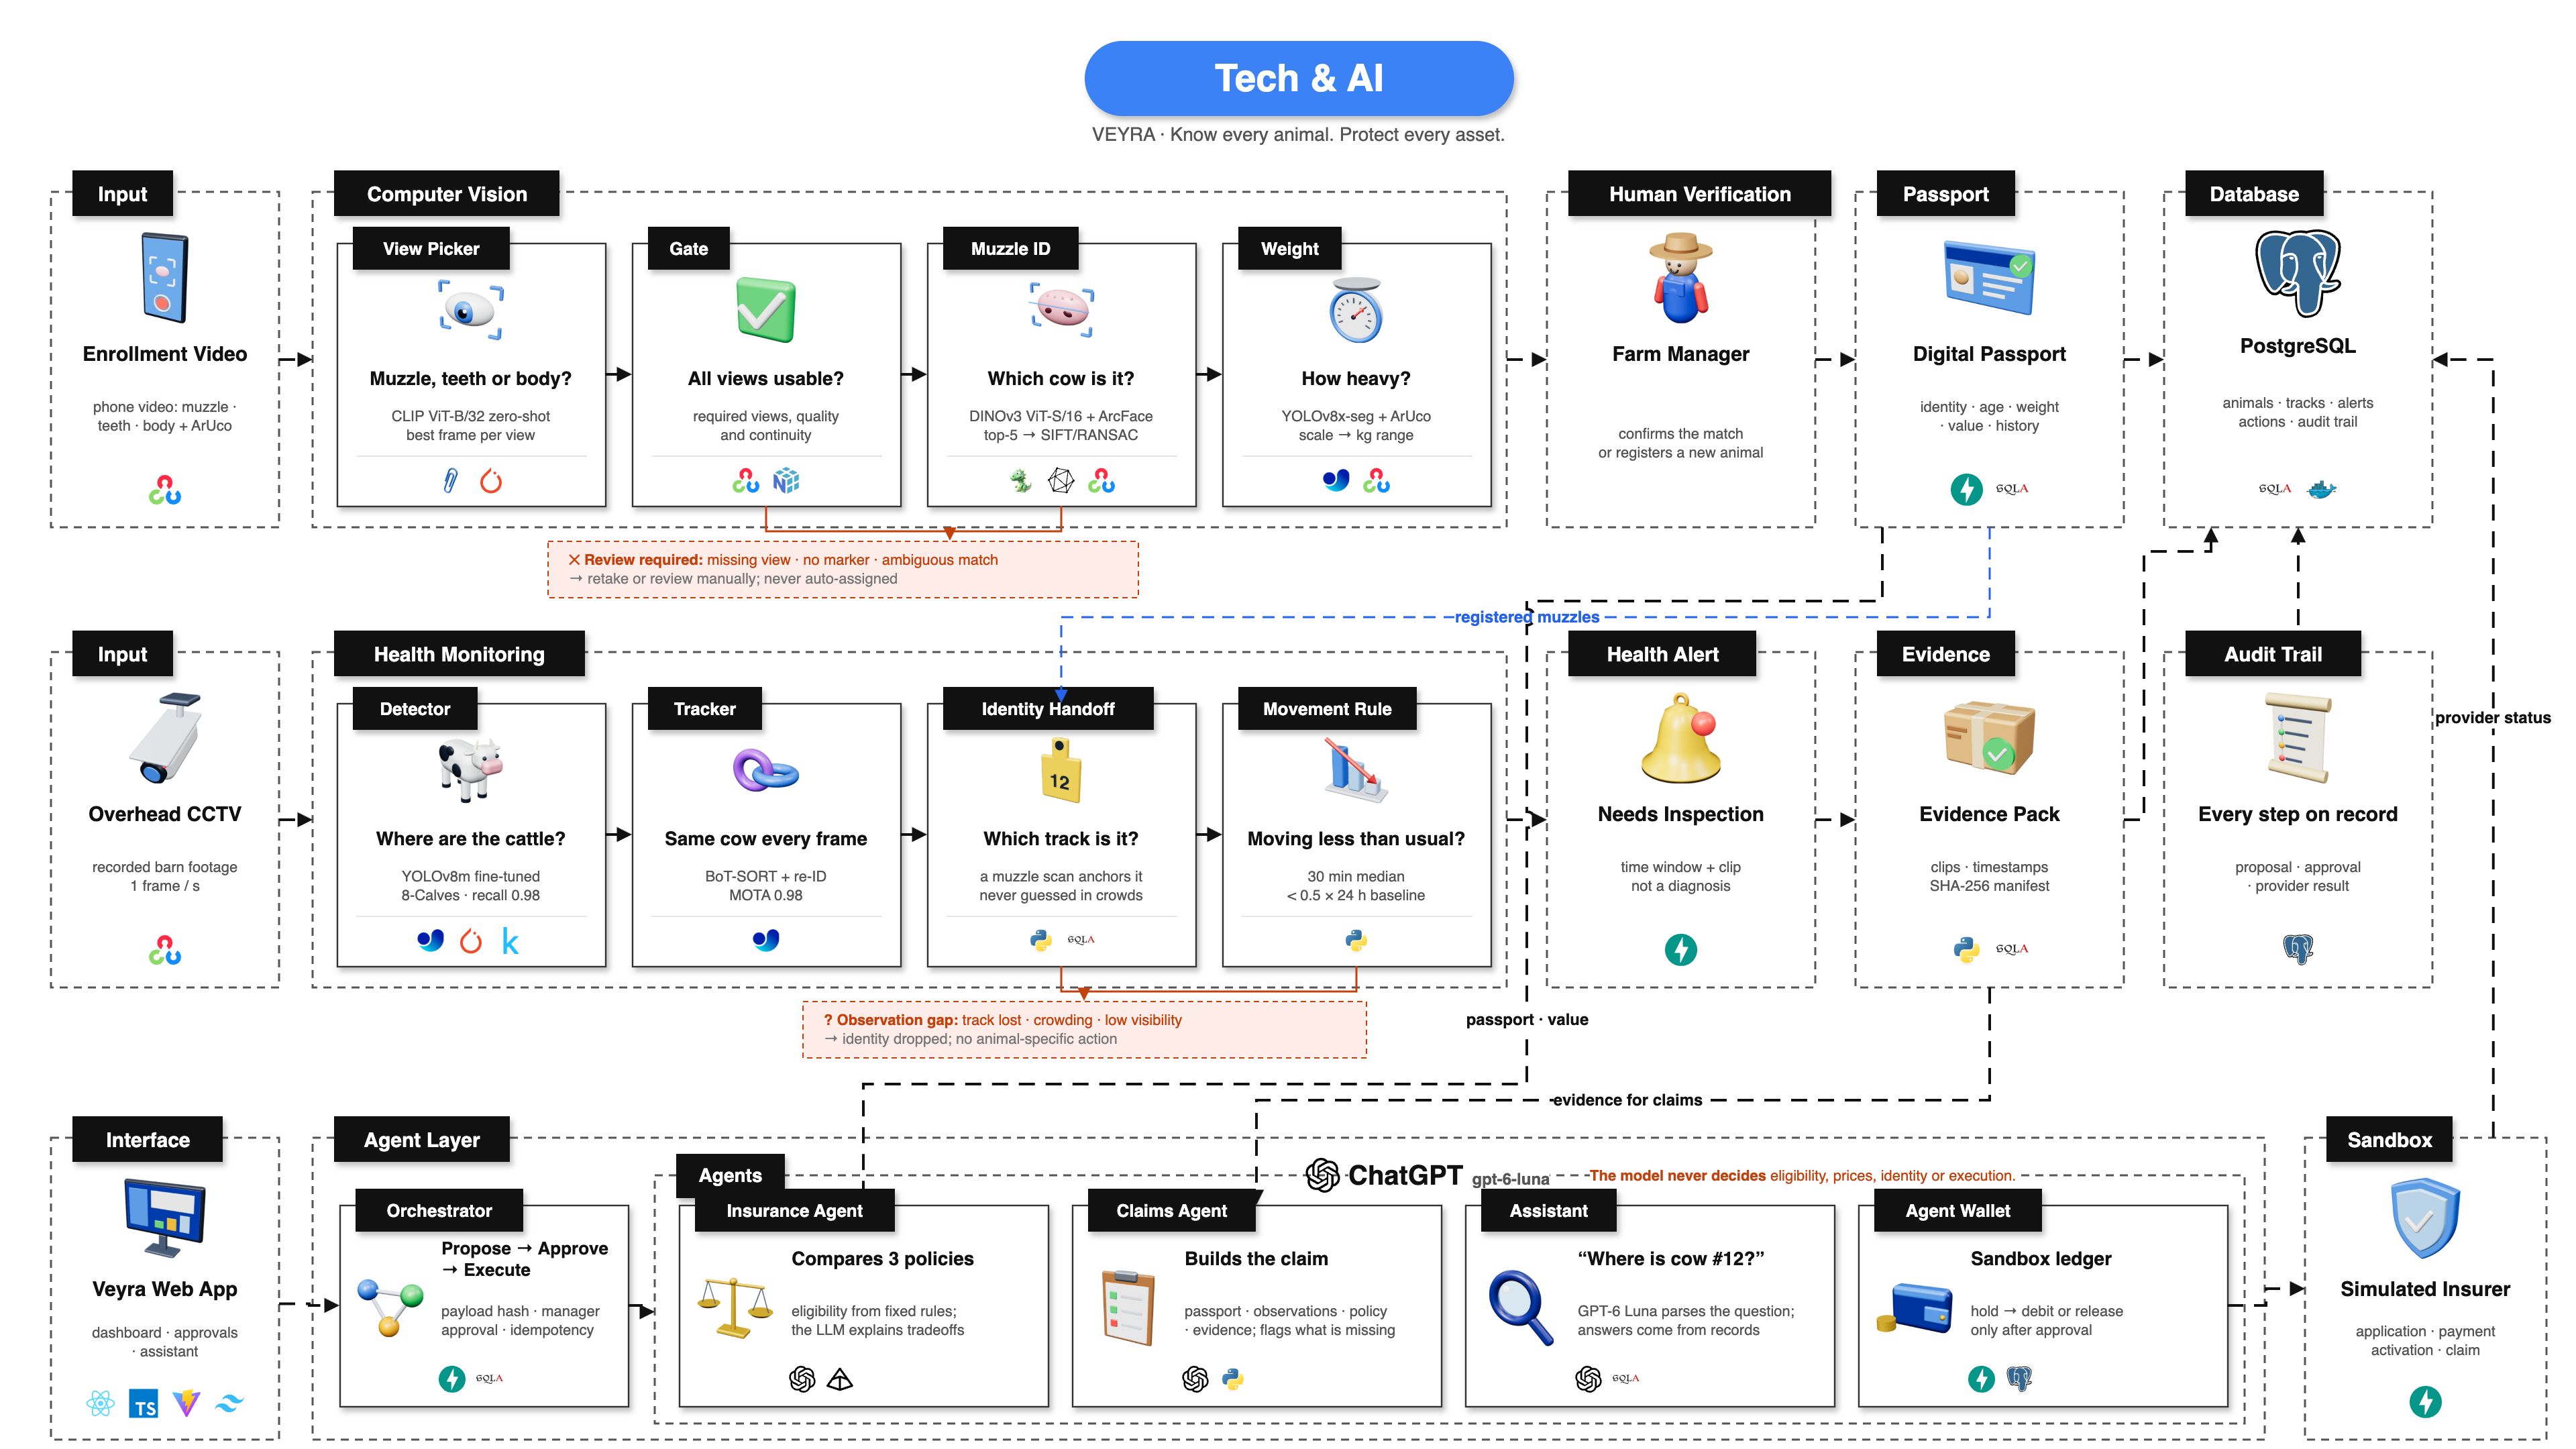
\includegraphics[width=\textwidth]{figures/architecture.png}
\caption{VEYRA system architecture: enrollment computer vision (top), camera health monitoring (middle), and the agent layer with the approval-gated wallet (bottom). Logos mark the technology behind each component.}
\label{fig:arch}
\end{figure}

\subsection{Guided Enrollment and View Selection}

The operator records one continuous video that follows on-screen prompts through the muzzle, the open mouth, and the full body side view, with a printed ArUco marker held flat against the flank (Figure~\ref{fig:enroll}). Each sampled frame $x$ is classified zero-shot with OpenCLIP ViT-B/32 \cite{radford2021clip,cherti2023openclip} against text prompts $t_k$ for the views $k \in \{\text{muzzle}, \text{teeth}, \text{body}, \text{other}\}$,
\begin{equation}
p(k \mid x) = \frac{\exp\!\big(\gamma \cos(g(x), h(t_k))\big)}{\sum_{k'} \exp\!\big(\gamma \cos(g(x), h(t_{k'}))\big)},
\end{equation}
where $g$ and $h$ are the image and text encoders and $\gamma$ is CLIP's logit scale. The best frame per view is kept, and side versus front or rear body views are separated by the aspect ratio of the cow detector's box. A quality gate then checks that every required view is present, usable, and recorded in one continuous take, with a live capture-quality meter guiding the operator; a missing view or marker returns a precise retake instruction instead of a guess. The muzzle crop uses the exact guide box shown on the capture screen (90\% of the frame width, aspect 1.18), so what the operator frames is what the matcher sees.

\subsection{Open-Set Muzzle Identification}

Identification is retrieval against the farm's gallery of registered animals, so it must also recognise animals it has never seen. The embedding network $f$ is a DINOv3 ViT-S/16 backbone \cite{simeoni2025dinov3} whose last four blocks are fine-tuned with the ArcFace loss \cite{deng2019arcface},
\begin{equation}
\mathcal{L} = -\log \frac{e^{s\cos(\theta_{y}+m)}}{e^{s\cos(\theta_{y}+m)} + \sum_{j\neq y} e^{s\cos\theta_{j}}}, \qquad s = 30,\ m = 0.30,
\end{equation}
producing an L2-normalised 512-dimensional embedding exported to ONNX. For a query muzzle $q$, the five gallery animals with the highest cosine similarity form the shortlist $S(q)$. Each candidate $a \in S(q)$ is then verified geometrically: SIFT keypoints on CLAHE-equalised images are matched with Lowe's ratio test (0.75) and filtered by a RANSAC homography, giving $n(q,a)$ verified inliers. The decision rule is
With $a^{*} = \arg\max_{a \in S(q)} n(q,a)$ the best-supported candidate,
\begin{equation}
\text{outcome} =
\begin{cases}
\text{uncertain} & \text{if } Q(q) < 0.6 \ \text{or}\ \exists a' \neq a^{*}: n(q,a') \ge 0.8\, n(q,a^{*}),\\
\text{candidate } a^{*} & \text{else if } n(q,a^{*}) > 5,\\
\text{new animal} & \text{otherwise,}
\end{cases}
\end{equation}
where $Q(q)$ is the quality of the muzzle crop and a rival within 80\% of the best inlier count makes the match ambiguous.
The embedding contributes ranking accuracy, while geometric verification contributes a threshold that transfers from validation to test animals. Every outcome is presented to the manager as a candidate with its evidence (closest animal and verified points), and a duplicate candidate must be linked or justified before a new passport is created.

\subsection{Weight Measurement and Indicative Value}

From the body frame, a YOLOv8x segmentation mask isolates the animal; its orientation and landmarks give pixel measurements, and the ArUco marker converts pixels to centimetres. The image path predicts weight from withers height $H$ with a log-linear model calibrated on tape-measured cattle,
\begin{equation}
\hat{W} = \exp(-4.4177 + 2.2109 \ln H) \ \text{kg}, \qquad [W_{\text{lo}}, W_{\text{hi}}] = \hat{W}\,(1 \mp b), \quad b = 0.121,
\end{equation}
where $b$ is the 80th percentile of out-of-fold relative error, so the range reflects measured accuracy rather than stacked assumptions. When a tape heart girth $G$ is available, the tape path averages Schaeffer's formula $W = G^{2} L / 10838$ (cm) and a locally recalibrated Crevat formula $W = 75.8\,G^{3}$ (m), with body length $L = 0.9133H + 43.36$; it uses the tighter band $b = 0.097$ and requests review when the two formulas disagree by more than 15\%. The indicative value of each end of the range is
\begin{equation}
V_{\{\text{lo},\text{hi}\}} = \big\lfloor W_{\{\text{lo},\text{hi}\}} \times p \big\rfloor,
\end{equation}
with $p$ a dated unit price in minor currency units per kilogram. Every estimate is stored with its method, version, source, and timestamp, and every confirmation creates a new version, so the passport always shows where a number came from.

\subsection{Insurance Advisory}

Eligibility is computed by deterministic rules over facts gathered from the passport. Each catalog rule $r$ evaluates to pass, fail, or unknown, where unknown means the fact is missing or an estimated range straddles the limit. For a product with rules $R$,
\begin{equation}
\text{eligibility} =
\begin{cases}
\text{ineligible} & \text{if } \exists r \in R: r = \text{fail},\\
\text{unknown (with the review needed)} & \text{else if } \exists r \in R: r = \text{unknown},\\
\text{eligible} & \text{otherwise.}
\end{cases}
\end{equation}
The insured value is the lower bound of the confirmed value range, and the annual premium is the product's rate applied to it, rounded half up. The agent recommends the eligible product with the lowest premium and cites the terms reference behind every reason. GPT-6 Luna then explains the computed outcomes in plain language through structured outputs. Its answer is checked against the inputs: explanations for products that were not supplied are dropped and terms references that do not exist in the catalog are removed, so the explanation can clarify a decision but never change one. Without the model, a deterministic template states the same facts.

\subsection{Camera Health Monitoring}

\paragraph{Detection and tracking.} Barn frames are processed by \texttt{calf\_detector\_v1}, a COCO-pretrained YOLOv8m fine-tuned on 500 hand-labelled frames of the 8-Calves barn \cite{fang2025eightcalves} on Kaggle (two NVIDIA T4 GPUs), and detections are linked by BoT-SORT with appearance re-identification \cite{aharon2022botsort}. When a generic COCO detector is used instead, only animal classes are kept, so people in the pen are never tracked.

\paragraph{Muzzle-anchored identity.} A track becomes associated with an animal only through a muzzle match that passes the identification bar (more than five inliers, quality at least 0.6, a confirmed animal of the same farm) or an explicit human assignment. On a camera with a calibrated scan zone $Z$, a muzzle scan at time $t_s$ hands the identity to the track whose box centre lies in the zone, provided it is the only one present:
\begin{equation}
\text{track } i \leftarrow \text{animal } a \iff \big|\{\, j : c(b_j(t_s)) \in Z,\ t_s - t_j^{\text{last}} \le 1\,\text{s} \,\}\big| = 1 \ \text{and } i \text{ is that track}.
\end{equation}
If two animals stand in the zone, nothing is handed over and both tracks become uncertain, so a crowded scan can never mislabel an animal.

\paragraph{Identity continuity (\texttt{handoff\_v2}).} An associated track keeps its identity only while continuity is reliable. With $\Delta_i(t)$ the time since track $i$ was last observed, the identity is released when
\begin{equation}
\Delta_i(t) > 1.0\,\text{s} \quad\text{or}\quad \exists j \ne i:\ \mathrm{IoU}\big(b_i, b_j\big) > 0.6 \ \text{for at least } 0.25\,\text{s}.
\end{equation}
An overlap release counts from the start of the overlap, and observations stored since then are downgraded to uncertain. A released identity is never re-attached automatically, so the system always prefers \emph{uncertain} to \emph{wrong}. The parameters were selected by a grid search over 120 combinations on real barn footage with a safety-first objective: fewest wrong identities in the worse segment, then most correct identities (Section~\ref{sec:continuity}).

\paragraph{Movement rule.} For each associated track and window $w$, the speed $v_w$ is the mean centroid displacement per second between consecutive frames in normalised frame units. A window is usable when mean visibility is at least 0.6 and frame coverage at least 0.7; otherwise it raises an observation-quality warning instead of a judgement. Against the animal's own baseline window on the same camera, $v_{\text{base}}$,
\begin{equation}
\text{reduced movement} \iff v_w < v_{\text{base}}\,(1 - \lambda), \qquad \lambda = 0.6,
\end{equation}
with one alert per animal, camera, and kind within a ten-minute cooldown. Each alert carries its observation window, the baseline window, the measured drop, the camera, and the clip reference, and recommends an inspection. The camera gallery is versioned from the confirmed animals and their muzzle references, so the manager can see whether every camera has acknowledged the latest gallery.

\subsection{Agent Wallet and Action Lifecycle}

The agent prepares four action types: policy application, premium payment, insurer notification, and claim submission. The server, not the client, builds each payload from current records and fixes it with a canonical hash,
\begin{equation}
h = \mathrm{SHA256}\big(\mathrm{canonical\_json}(\text{payload})\big).
\end{equation}
Only a manager can approve, and the approval must name the exact hash and version that were reviewed. An action expires 30 minutes after it is proposed. Before execution the payload is rebuilt from current records; any change to amount, recipient, terms, animal, or evidence cancels the approval as stale. Execution requires an idempotency key and runs as three short steps, never holding a write transaction across the provider call: (1) check state, expiry, freshness, and funds, insert the execution record, and place a hold on the sandbox balance; (2) call the provider, which stores its result under the key; (3) apply the result, posting the debit and releasing the hold on success, or only releasing it on decline. A timeout leaves the hold in place, and a retry with the same key reconciles from the provider's record, so a payment can never be made twice. A successful premium payment marks the policy as paid and pending activation, and the policy becomes active only when the insurer separately confirms it. The agent's proposal, the manager's decision, and the provider's result are three distinct audit events.

\subsection{Incidents and Claims}

An incident keeps the camera's observations, the farmer's report, and the veterinarian's professional findings in separate fields, and an alert alone never creates a claim. A claim draft requires an active policy whose covered perils include the incident, and its checklist is built from the product's claim requirements: passport reference, linked camera observation, incident facts, farmer declaration, and veterinary assessment. For every death claim the system adds a biometric requirement: a fresh muzzle scan of the carcass is matched against the claimed animal's enrolled references \emph{and} every other confirmed animal on the farm. A match satisfies the requirement, a different animal is reported by name, and an ambiguous or low-detail scan asks for a retake. A claim submission with any missing item is refused with the list of what is missing, and a newer identity check or finding after approval makes the approved submission stale. Approved submissions return a sandbox receipt with an assessment-pending status.

\subsection{Conversational Agent and Assistant}

The in-app VEYRA agent guides three journeys: finding insurance for an uninsured animal, filing a claim for an insured one, and tracking a claim's status. Each turn reads the records again and replies with typed, data-backed cards such as a passport summary, plan comparison, application draft, action review, claim checklist, and receipt. It asks at most three short questions, only where a fact is missing. The agent prepares and never approves: an action-review card points to a pending action that only a manager can stamp. The farmer's text is treated strictly as data and never as an instruction. The assistant answers questions such as ``Where was animal-demo-001 last seen, and what coverage is active?'' in two steps: GPT-6 Luna parses the question into a validated intent, and the answer is written from the farm's records, one fact per value, each linked to its source record. Location answers state the camera and the time of the last associated observation and note when that observation is more than an hour old.

\subsection{Implementation}

Figure~\ref{fig:stack} summarises the technology. The backend is a FastAPI service with 61 endpoints across 21 route modules, Pydantic schemas, and SQLAlchemy~2 persistence; the CCTV pipeline service runs on PostgreSQL. The API contract is exported as OpenAPI, and the web client generates its TypeScript types from it, so the two cannot drift. The web app uses React~19, TypeScript, Vite, Tailwind CSS~4, TanStack Query, and React Router; it is installable as a progressive web app and is designed for tablets in daylight, with high contrast and large touch targets. Role-based access separates the manager (approves and declines), the operator (enrolls and reviews tracks), the veterinarian (adds findings, no payment authority), and the assessor (reads submissions). A perception facade selects each ML capability independently and labels every output \texttt{live}, \texttt{prototype}, \texttt{simulated}, or \texttt{documented}, so the interface always states the provenance of a result. The whole platform ships as one Docker image. All computer-vision models were trained on Kaggle with two NVIDIA T4 GPUs, and the muzzle embedding is served with ONNX Runtime.

\subsection{Datasets}

Every model is trained and evaluated on public, openly licensed data that matches its task (Table~\ref{tab:datasets}, Figure~\ref{fig:datasets}). Each dataset is split by the unit that must generalise: by animal for identification, so test animals are new identities; by recording day for detection, so the detector is scored on a day it never saw; and by fold for the weight calibration.

\begin{table}[H]
\centering
\caption{Datasets used for training and evaluation.}
\label{tab:datasets}
\footnotesize
\setlength{\tabcolsep}{4pt}
\begin{tabularx}{\textwidth}{>{\raggedright\arraybackslash}p{3.1cm}>{\raggedright\arraybackslash}p{2.3cm}>{\raggedright\arraybackslash}X>{\raggedright\arraybackslash}X}
\toprule
Dataset & Task & Content & Split \\
\midrule
Beef Cattle Muzzle database \cite{li2022muzzle} (CC BY 4.0) & Muzzle identification & 4{,}923 cropped muzzle photographs of 268 US feedlot cattle & By animal: 134 training animals; 54 validation and 80 test animals, each with a registered gallery and unknown animals (1{,}326 test queries) \\
8-Calves \cite{fang2025eightcalves} (CC BY 4.0) & Detection and tracking & One hour of overhead barn CCTV of eight Holstein Friesian calves, 800$\times$600 at 20~fps, with hand-labelled frames and identity-labelled tracks & By recording day: 500 training frames, 100 validation frames (782 calves); held-out test session \texttt{pmfeed\_4\_3\_16} (12{,}000 frames) \\
Cattle side and back view, R11 \cite{mendeley_r11} (CC BY 4.0) & Weight calibration & 71 side photographs of Simmental-cross cattle with tape-measured withers height, heart girth, body length, and scale weight (341--644\,kg) & 6-fold cross-validation, seed 42 \\
\bottomrule
\end{tabularx}
\end{table}

\begin{figure}[H]
\centering
\begin{subfigure}[b]{0.36\textwidth}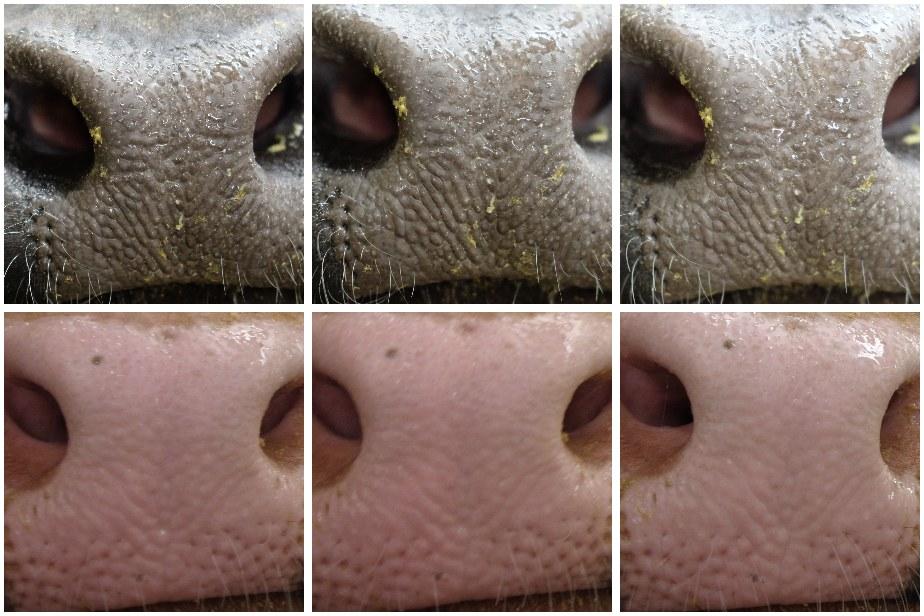
\includegraphics[width=\textwidth]{figures/data_muzzle.jpg}\caption{Muzzle database: two animals, three photographs each}\end{subfigure}\hfill
\begin{subfigure}[b]{0.33\textwidth}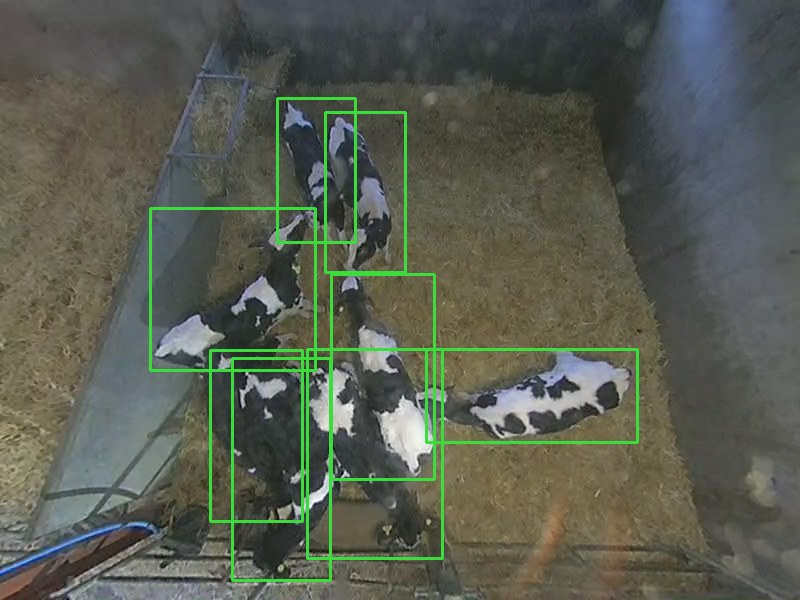
\includegraphics[width=\textwidth]{figures/data_8calves.jpg}\caption{8-Calves: hand-labelled frame with calf boxes}\end{subfigure}\hfill
\begin{subfigure}[b]{0.28\textwidth}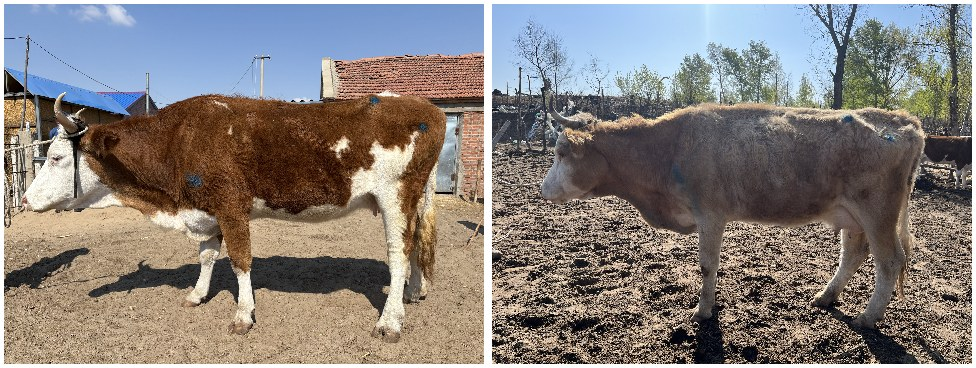
\includegraphics[width=\textwidth]{figures/data_r11.jpg}\caption{R11: side views for weight}\end{subfigure}
\caption{Samples from the training datasets. Each row of (a) is one animal: the ridge-and-bead pattern is stable within an animal and distinct between animals, which is what the matcher learns. Frames in (b) show the constant contact and occlusion that make identity preservation hard.}
\label{fig:datasets}
\end{figure}

\subsection{Training Procedure}

All training runs on Kaggle with two NVIDIA T4 GPUs from notebooks generated by versioned builder scripts, with a fixed seed of 42, so every run is reproducible end to end. Table~\ref{tab:training} summarises the configurations.

\paragraph{Muzzle embedding.} The backbone is \texttt{vit\_small\_patch16\_dinov3.lvd1689m} from timm at 224$\times$224. The early blocks stay frozen to preserve DINOv3's general features; the last four transformer blocks, a 512-dimensional projection with batch normalisation, and the ArcFace head are trained on the 134 training animals only. Augmentation imitates frames from a handheld phone video: random resized crops (scale 0.7--1.0, aspect 0.85--1.18, matching the capture guide), rotations up to 15\textdegree, brightness and contrast jitter of 0.3, saturation jitter of 0.2, and Gaussian blur with probability 0.3. The optimiser is AdamW with separate learning rates for the backbone ($2\times10^{-5}$) and the new layers ($10^{-3}$), weight decay 0.05, one warmup epoch followed by cosine decay, and mixed precision; each batch of 64 is split across both GPUs with \texttt{DataParallel}. After every epoch the model is scored on the validation animals with the same open-set protocol used for testing, and the checkpoint with the best open-set result is kept (epoch 13 of 20). The selected model is exported to ONNX with a dynamic batch axis. In the same notebook, SIFT/RANSAC, DINOv2 and DINOv3 zero-shot, and the fine-tuned embedding are scored on identical animals, which produces the leaderboard in Table~\ref{tab:muzzle}.

\paragraph{Calf detector.} \texttt{calf\_detector\_v1} starts from COCO-pretrained YOLOv8m and is trained as a single class at 800\,px on the 500 training frames. Mosaic augmentation multiplies the variety of crowding patterns and is switched off for the last 15 epochs so that the model finishes on whole frames; horizontal and vertical flips (0.5), rotations up to 10\textdegree, and HSV value and saturation jitter of 0.3 add robustness to camera angle and lighting. Training uses a cosine learning-rate schedule, a batch of 16 across both GPUs, and early stopping with a patience of 30 epochs: the run stopped at epoch 102 with the best weights at epoch 72. The zero-shot COCO model is scored on the same validation frames before training, so the gain from fine-tuning is measured directly.

\paragraph{Weight models.} The withers-height log-linear model, the body-length regression ($L = 0.9133H + 43.36$), and the recalibrated Crevat constant (75.8 instead of 80) are fitted on R11 with 6-fold cross-validation. Every reported error and every range band is computed out of fold, so the ranges a farm manager sees reflect measured, not assumed, accuracy.

\paragraph{Continuity policy.} \texttt{handoff\_v2} is selected by a grid search over the maximum gap $\{0.5, 1, 2, 5\}$\,s, the crowding IoU $\{0.3, 0.4, 0.5, 0.6, 0.7\}$, and the crowding duration $\{0.25, 0.5, 0.75, 1, 2, \text{off}\}$\,s on the tracked test session; the script runs the production policy code itself, so the tuned rule is exactly the deployed rule.

\begin{table}[H]
\centering
\caption{Training configurations (Kaggle, 2$\times$ NVIDIA T4, seed 42).}
\label{tab:training}
\footnotesize
\setlength{\tabcolsep}{4pt}
\begin{tabularx}{\textwidth}{>{\raggedright\arraybackslash}p{3.0cm}>{\raggedright\arraybackslash}X>{\raggedright\arraybackslash}X}
\toprule
Setting & Muzzle embedding & Calf detector \\
\midrule
Base model & DINOv3 ViT-S/16 (LVD-1689M), timm & YOLOv8m, COCO-pretrained \\
Trainable part & Last 4 blocks + 512-d projection + ArcFace head & Full network, single class \\
Input size & 224$\times$224 & 800\,px \\
Objective & ArcFace, $s = 30$, $m = 0.30$ & YOLOv8 box, class, and DFL losses \\
Optimiser and schedule & AdamW, LR $2\times10^{-5}$ backbone / $10^{-3}$ head, weight decay 0.05, 1 warmup epoch + cosine & Ultralytics default optimiser, cosine LR \\
Batch and epochs & 64 (32 per GPU), 20 epochs, best epoch 13 & 16 (8 per GPU), up to 120 epochs, patience 30, best epoch 72 \\
Augmentation & Resized crop, rotation 15\textdegree, colour jitter, Gaussian blur & Mosaic (off for last 15 epochs), flips, rotation 10\textdegree, HSV jitter \\
Model selection & Best open-set result on validation animals & Best validation fitness (mAP) \\
Export & ONNX, dynamic batch & Ultralytics \texttt{.pt} \\
\bottomrule
\end{tabularx}
\end{table}

\subsection{Evaluation Protocol}

Every model was evaluated on data it never saw during training or threshold selection. The muzzle matcher uses an animal-level split of the Beef Cattle Muzzle database \cite{li2022muzzle}, so test animals are new identities, and its acceptance threshold is chosen on validation animals at an unknown-animal false-match rate of at most 5\% and reported once on test animals. The detector is split by recording day, and tracking is scored on the held-out test session \texttt{pmfeed\_4\_3\_16} of 8-Calves (12{,}000 frames, ten minutes at 20~fps) with MOTA \cite{bernardin2008mota} and IDF1 \cite{ristani2016idf1}. Weight is evaluated with 6-fold cross-validation on 71 side photographs of tape-measured cattle \cite{mendeley_r11}. The platform's behaviour is verified by automated tests.

\section{Results and Discussion}

\subsection{Muzzle Identification}

Table~\ref{tab:muzzle} reports identification on held-out test animals. Fine-tuning with ArcFace lifts the embedding to 96.6\% rank-1 and 97.6\% top-5, above both the DINOv3 and DINOv2 zero-shot baselines, which makes it an excellent shortlist. Geometric verification then turns that shortlist into a decision: the hybrid keeps 92.5\% correct matches while cutting the false-match rate on unknown animals from 32.4\% to 1.4\%. This is the property that matters for a registry: an animal that has never been enrolled is reported as new rather than silently matched to someone else's cow. Run end to end through the production adapter on 974 registered and 352 unknown test queries, the matcher returns the correct animal for 92.5\% of registered queries with only 0.4\% wrong candidates, and reports 98.9\% of unknown animals as new.

\begin{table}[H]
\centering
\caption{Muzzle identification on held-out test animals (animal-level split).}
\label{tab:muzzle}
\small
\setlength{\tabcolsep}{3.5pt}
\begin{tabular}{lccccc}
\toprule
Method & Rank-1 & Top-5 & \makecell{Correct match\\at threshold} & \makecell{Wrong match\\(registered)} & \makecell{Unknown\\false} \\
\midrule
\textbf{Hybrid (embedding + SIFT/RANSAC)} & 0.927 & 0.927 & \textbf{0.925} & 0.005 & \textbf{0.014} \\
DINOv3 + ArcFace, cosine only & \textbf{0.966} & \textbf{0.976} & 0.952 & 0.005 & 0.324 \\
SIFT + RANSAC only & 0.925 & 0.925 & 0.924 & 0.001 & 0.017 \\
DINOv3 ViT-S/16 zero-shot & 0.939 & 0.961 & 0.843 & 0.002 & 0.145 \\
DINOv2 ViT-S/14 zero-shot & 0.925 & 0.953 & 0.827 & 0.007 & 0.153 \\
\bottomrule
\end{tabular}
\end{table}

\subsection{Cattle Detection and Tracking}

Fine-tuning turned detection from the bottleneck into a solved step (Table~\ref{tab:detector}): recall on a held-out recording day rose from 0.254 for the COCO detector to 0.978, with precision 0.936 and mAP50 0.987.

\begin{table}[H]
\centering
\caption{Detection on a held-out validation day of 8-Calves (100 frames, 782 calves).}
\label{tab:detector}
\small
\begin{tabular}{lcccc}
\toprule
Detector & Precision & Recall & mAP50 & mAP50--95 \\
\midrule
COCO YOLOv8m, animal classes & 0.777 & 0.254 & -- & -- \\
\textbf{\texttt{calf\_detector\_v1} (fine-tuned YOLOv8m)} & \textbf{0.936} & \textbf{0.978} & \textbf{0.987} & \textbf{0.604} \\
\bottomrule
\end{tabular}
\end{table}

On ten minutes of the held-out test session, the fine-tuned detector with BoT-SORT re-identification reaches recall 0.997, MOTA 0.976, and IDF1 0.709, the best identity preservation of every combination tested (Table~\ref{tab:tracking}). For reference, the 8-Calves benchmark reports IDF1 of about 0.27 for the trackers it evaluates on the same barn \cite{fang2025eightcalves}.

\begin{table}[H]
\centering
\caption{Tracking on the held-out 8-Calves test session (12{,}000 frames).}
\label{tab:tracking}
\small
\begin{tabular}{lcccc}
\toprule
Detector + tracker & Recall & MOTA & IDF1 & ID switches \\
\midrule
COCO + ByteTrack & 0.405 & 0.319 & 0.136 & 751 \\
COCO + BoT-SORT re-ID & 0.410 & 0.323 & 0.160 & 735 \\
\texttt{calf\_detector\_v1} + ByteTrack & 0.997 & 0.977 & 0.666 & 143 \\
\texttt{calf\_detector\_v1} + BoT-SORT & 0.997 & 0.977 & 0.668 & 116 \\
\textbf{\texttt{calf\_detector\_v1} + BoT-SORT re-ID} & \textbf{0.997} & \textbf{0.976} & \textbf{0.709} & 120 \\
\bottomrule
\end{tabular}
\end{table}

\subsection{Identity Continuity}
\label{sec:continuity}

Table~\ref{tab:handoff} evaluates identity continuity after every calf's identity is handed to its track at the start of two five-minute segments, as the scan zone does. Keeping identities forever looks attractive but assigns a wrong identity to 2.3\% of observations after a single swap, and a naive overlap rule discards most identities. \texttt{handoff\_v2} keeps 67.6\% and 54.5\% of observations correctly identified with \textbf{zero wrong identities in both segments}; every remaining observation is explicitly uncertain, never mislabelled, and fewer than 0.4\% of calves were missed by the detector. For an insurance-grade record, this is the decisive guarantee: an alert or a claim can only ever attach to the right animal.

\begin{table}[H]
\centering
\caption{Identity continuity on real barn CCTV (share of labelled calf observations).}
\label{tab:handoff}
\small
\begin{tabular}{lcccc}
\toprule
Rule & \makecell{Min 0--5\\correct} & \makecell{Min 0--5\\wrong} & \makecell{Min 5--10\\correct} & \makecell{Min 5--10\\wrong} \\
\midrule
Keep identity forever & 0.704 & 0.000 & 0.679 & 0.023 \\
Drop on any overlap (IoU $>$ 0.3) & 0.103 & 0.000 & 0.182 & 0.000 \\
\textbf{\texttt{handoff\_v2} (gap 1.0\,s, IoU 0.6 for 0.25\,s)} & \textbf{0.676} & \textbf{0.000} & \textbf{0.545} & \textbf{0.000} \\
\bottomrule
\end{tabular}
\end{table}

On the AI-generated demonstration footage (Figure~\ref{fig:cctv}), the same pipeline tracked every calf in the pen while excluding the handler, and the scan on the yellow mat handed the enrolled calf's identity to exactly one track, which held it to the end of the clip while the other calves remained unidentified.

\subsection{Weight Estimation}

Table~\ref{tab:weight} reports out-of-fold weight accuracy. The image path halves the error of a population-mean baseline (8.7\% versus 15.8\% MAPE) with almost no bias, and the tape path reaches 5.4\% MAPE with 86\% of animals within 10\% of their scale weight. On the same cattle, Schaeffer's formula applied to tape measurements reaches 5.7\% MAPE with 90\% of animals within 10\%, confirming that the measurement pipeline is anchored on well-established zootechnical formulas.

\begin{table}[H]
\centering
\caption{Weight estimation, 6-fold cross-validation on tape-measured cattle (341--644\,kg).}
\label{tab:weight}
\small
\begin{tabular}{lcccc}
\toprule
Method & MAPE & Bias & Within 10\% & 80\% band \\
\midrule
Predict the mean (baseline) & 15.8\% & +3.4\% & 44\% & $\pm$22.6\% \\
\textbf{Image path: withers height, log-linear} & \textbf{8.7\%} & \textbf{+0.2\%} & 59\% & $\pm$12.1\% \\
\textbf{Tape path: heart girth, Schaeffer + Crevat} & \textbf{5.4\%} & \textbf{+0.9\%} & \textbf{86\%} & $\pm$9.7\% \\
\bottomrule
\end{tabular}
\end{table}

\subsection{System Integrity}

The platform's guarantees are encoded as automated tests: 551 backend tests and 135 web test cases pass. Table~\ref{tab:guarantees} lists representative properties and the behaviour the tests verify. The complete demonstration journey, from a fresh herd through enrollment, valuation, policy activation, a camera alert, a claim, and the audit review, runs in about 25 seconds of application time.

\begin{table}[H]
\centering
\caption{Representative guarantees verified by automated tests.}
\label{tab:guarantees}
\small
\begin{tabularx}{\textwidth}{>{\raggedright\arraybackslash}p{4.6cm}X}
\toprule
Guarantee & Verified behaviour \\
\midrule
No duplicate money movement & A charge is idempotent per key; a reused or new key after success is rejected as a duplicate. \\
Approval binds one payload & Declined, expired, or stale approvals cannot execute; a new valuation after approval cancels the payment. \\
Failed payments are safe & A declined payment fails and releases its hold; a timeout reconciles from the provider record. \\
No forced identity & A crowded scan identifies nobody and raises no animal alert; an empty zone identifies nobody. \\
Claim integrity & A missing veterinary assessment blocks submission; a later identity mismatch makes an approved submission stale. \\
Grounded answers & Location answers state camera and time and flag stale observations as an observation gap. \\
\bottomrule
\end{tabularx}
\end{table}

\subsection{Responsible AI by Design}

Responsibility is built into the architecture rather than added to the prompt. The language model explains and parses; it never decides eligibility, prices, identity, or execution, and its outputs are grounded against the records before display. Uncertainty is a first-class state: unassigned, ambiguous, missing, and stale conditions receive the same design care as success states, and the system prefers \emph{uncertain} to \emph{wrong} at every step, from the muzzle matcher to the continuity policy. Every number on screen shows its source, unit, date, and method, and every output carries its provenance label. Alerts request inspections and leave diagnosis to veterinarians. Financial actions require an explicit, hash-bound manager approval, and the audit trail separates what the agent proposed, what the manager decided, and what the provider returned.

\subsection{Scalability and Production Readiness}

\paragraph{Adoption path.} VEYRA fits the existing farm workflow: the operator already handles the animal for tagging and health checks, and one short guided video completes enrollment within that routine. The manager's work shrinks from reconciling separate records to reviewing one passport and stamping prepared actions.

\paragraph{Integration readiness.} Insurers, payment providers, and cameras sit behind adapters with explicit, tested contracts (idempotent execution, separate activation, versioned camera galleries), so connecting a production partner replaces an adapter, not the approval logic. The open API contract lets insurers read submissions directly through a dedicated assessor role and leaves a clean integration point for livestock registries.

\paragraph{Deployment.} The platform runs as one container and is installable on tablets as a progressive web app. The muzzle model is exported to ONNX, which allows inference on modest hardware close to the barn, and every ML capability degrades independently to a labelled fallback so that the farm workflow never stops.

\paragraph{Roadmap.} The rollout proceeds in gated phases: partner discovery with farm managers, veterinarians, and insurers; an identity and valuation pilot with consented reference data; monitoring validation at an eye-level identification point; integration of one insurer's quotes, activation, and claim status; and controlled financial execution with a payment partner. Each phase advances on measured outcomes such as reconciliation time, identity-association precision, alert precision per animal-day, claim-preparation time, and duplicate-transaction count.

\section{Conclusion}

VEYRA shows that a single, biometrically anchored animal record can connect what a farm sees, what an animal is worth, and how it is protected. One guided phone video creates a Digital Livestock Passport with a confirmed muzzle identity and a measured weight range; barn cameras attach their observations to that passport only when identity is certain; and an AI agent turns the record into insurance applications, payments, and claims that execute only after a manager approves exactly what will happen. With 92.5\% correct muzzle identification and 98.9\% of unseen animals correctly reported as new, 0.978 detection recall, IDF1 0.709 on real barn footage, zero wrong identities under the continuity policy, and approval-bound, idempotent execution verified by more than 680 automated tests, VEYRA provides the trustworthy identity and evidence layer that makes livestock insurance faster to buy, easier to claim, and harder to defraud.

\begin{thebibliography}{99}
\small
\bibitem{ipb2025auts} Indonesian Journal of Agricultural Resource and Environmental Economics (2025). Article on the AUTS/K cattle and buffalo insurance programme and its regulatory basis. \url{https://journal.ipb.ac.id/ijaree/article/download/62492/32345/381654}
\bibitem{jae2022auts} Jurnal Agro Ekonomi (2022). Article on the AUTS/K premium and subsidy scheme. Ministry of Agriculture, Republic of Indonesia. \url{https://epublikasi.pertanian.go.id/berkala/jae/article/download/3438/3460/4611}
\bibitem{republika2019} Republika (2019). Asuransi pertanian beri ketenangan petani dan peternak, 7 June 2019. \url{https://ekonomi.republika.co.id/berita/psq23v453/asuransi-pertanian-beri-ketenangan-petani-dan-peternak}
\bibitem{kontan2018} Kontan (2018). 20.800 ekor sapi berhasil ikut asuransi. \url{https://industri.kontan.co.id/news/20800-ekor-sapi-berhasil-ikut-asuransi}
\bibitem{kumar2017muzzle} Kumar, S., Pandey, A., Satwik, K.S.R., Kumar, S., Singh, S.K., Singh, A.K. \& Mohan, A. (2018). Deep learning framework for recognition of cattle using muzzle point image pattern. \emph{Measurement} 116:1--17.
\bibitem{li2022muzzle} Li, G., Erickson, G.E. \& Xiong, Y. (2022). Individual beef cattle identification using muzzle images and deep learning techniques. \emph{Animals} 12(11):1453. Dataset: Zenodo record 6324361, CC BY 4.0.
\bibitem{simeoni2025dinov3} Sim\'eoni, O., Vo, H.V., Seitzer, M., et al. (2025). DINOv3. arXiv:2508.10104.
\bibitem{deng2019arcface} Deng, J., Guo, J., Xue, N. \& Zafeiriou, S. (2019). ArcFace: additive angular margin loss for deep face recognition. \emph{Proc. IEEE/CVF CVPR}, pp.~4690--4699.
\bibitem{lowe2004sift} Lowe, D.G. (2004). Distinctive image features from scale-invariant keypoints. \emph{International Journal of Computer Vision} 60(2):91--110.
\bibitem{fischler1981ransac} Fischler, M.A. \& Bolles, R.C. (1981). Random sample consensus: a paradigm for model fitting with applications to image analysis and automated cartography. \emph{Communications of the ACM} 24(6):381--395.
\bibitem{jocher2023yolov8} Jocher, G., Chaurasia, A. \& Qiu, J. (2023). Ultralytics YOLOv8. \url{https://github.com/ultralytics/ultralytics}
\bibitem{zhang2022bytetrack} Zhang, Y., Sun, P., Jiang, Y., et al. (2022). ByteTrack: multi-object tracking by associating every detection box. \emph{Proc. ECCV}.
\bibitem{aharon2022botsort} Aharon, N., Orfaig, R. \& Bobrovsky, B.-Z. (2022). BoT-SORT: robust associations multi-pedestrian tracking. arXiv:2206.14651.
\bibitem{fang2025eightcalves} Fang, X., Hannuna, S., Campbell, N. \& Simpson, E. (2025). 8-Calves image dataset. arXiv:2503.13777.
\bibitem{garrido2014aruco} Garrido-Jurado, S., Mu\~noz-Salinas, R., Madrid-Cuevas, F.J. \& Mar\'in-Jim\'enez, M.J. (2014). Automatic generation and detection of highly reliable fiducial markers under occlusion. \emph{Pattern Recognition} 47(6):2280--2292.
\bibitem{radford2021clip} Radford, A., Kim, J.W., Hallacy, C., et al. (2021). Learning transferable visual models from natural language supervision. \emph{Proc. ICML}.
\bibitem{cherti2023openclip} Cherti, M., Beaumont, R., Wightman, R., et al. (2023). Reproducible scaling laws for contrastive language-image learning. \emph{Proc. IEEE/CVF CVPR}.
\bibitem{bernardin2008mota} Bernardin, K. \& Stiefelhagen, R. (2008). Evaluating multiple object tracking performance: the CLEAR MOT metrics. \emph{EURASIP Journal on Image and Video Processing}.
\bibitem{ristani2016idf1} Ristani, E., Solera, F., Zou, R., Cucchiara, R. \& Tomasi, C. (2016). Performance measures and a data set for multi-target, multi-camera tracking. \emph{ECCV Workshops}.
\bibitem{mendeley_r11} Cattle side and back view images with body measurements and weight. Mendeley Data, h2s22wr5py, version 3, CC BY 4.0.
\end{thebibliography}

\newpage
\appendix
\section{Appendix A: Supporting Figures}

\begin{figure}[H]
\centering
\begin{subfigure}{0.32\textwidth}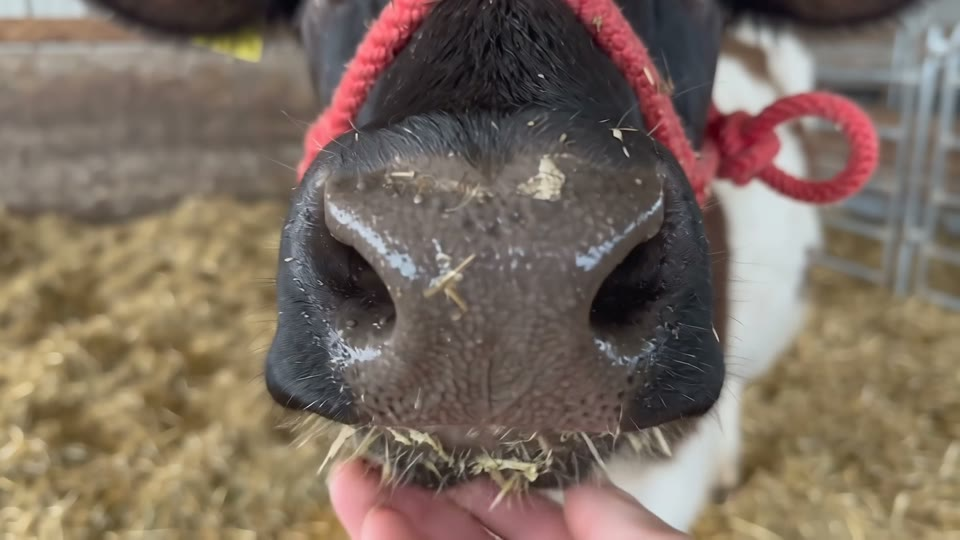
\includegraphics[width=\textwidth]{figures/enroll_muzzle.jpg}\caption{Muzzle view}\end{subfigure}\hfill
\begin{subfigure}{0.32\textwidth}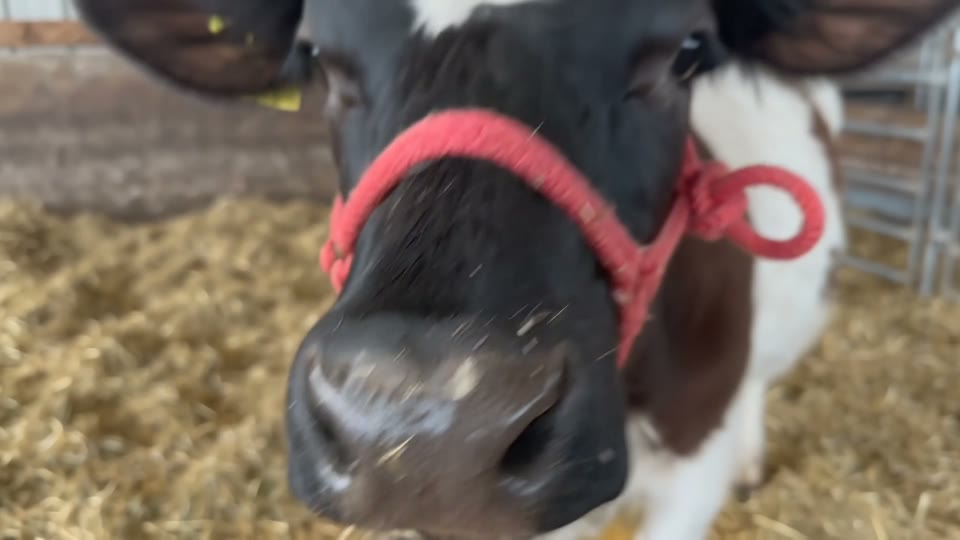
\includegraphics[width=\textwidth]{figures/enroll_face.jpg}\caption{Head view}\end{subfigure}\hfill
\begin{subfigure}{0.32\textwidth}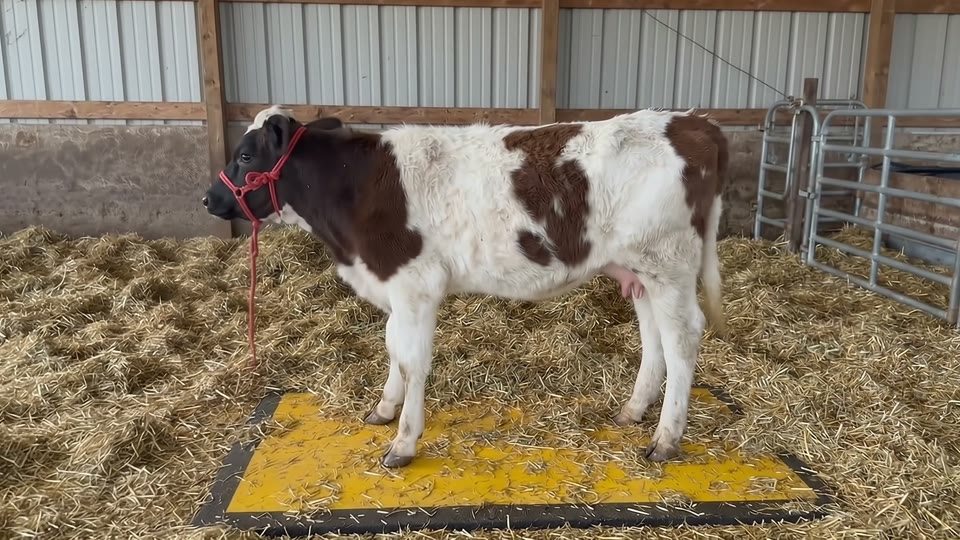
\includegraphics[width=\textwidth]{figures/enroll_body.jpg}\caption{Body side view}\end{subfigure}
\caption{Guided enrollment: one continuous phone video moves through the muzzle, head, and full side view. Frames from AI-generated (Google Veo) demonstration footage built from training-data references.}
\label{fig:enroll}
\end{figure}

\begin{figure}[H]
\centering
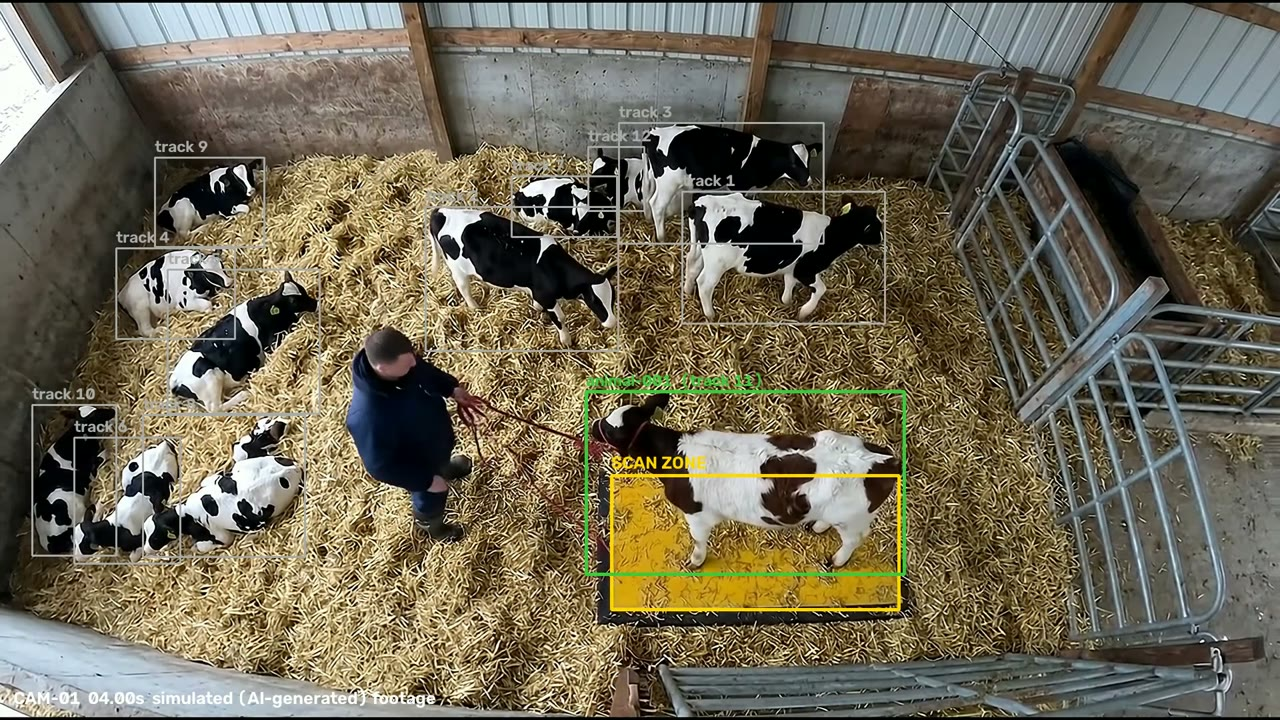
\includegraphics[width=0.92\textwidth]{figures/cctv_tracked.jpg}
\caption{Overhead barn CCTV with tracked calves and the calibrated scan zone (yellow). The scanned calf (green) receives the enrolled identity; the handler is never tracked. AI-generated demonstration footage processed by the real tracking pipeline.}
\label{fig:cctv}
\end{figure}

\begin{figure}[H]
\centering
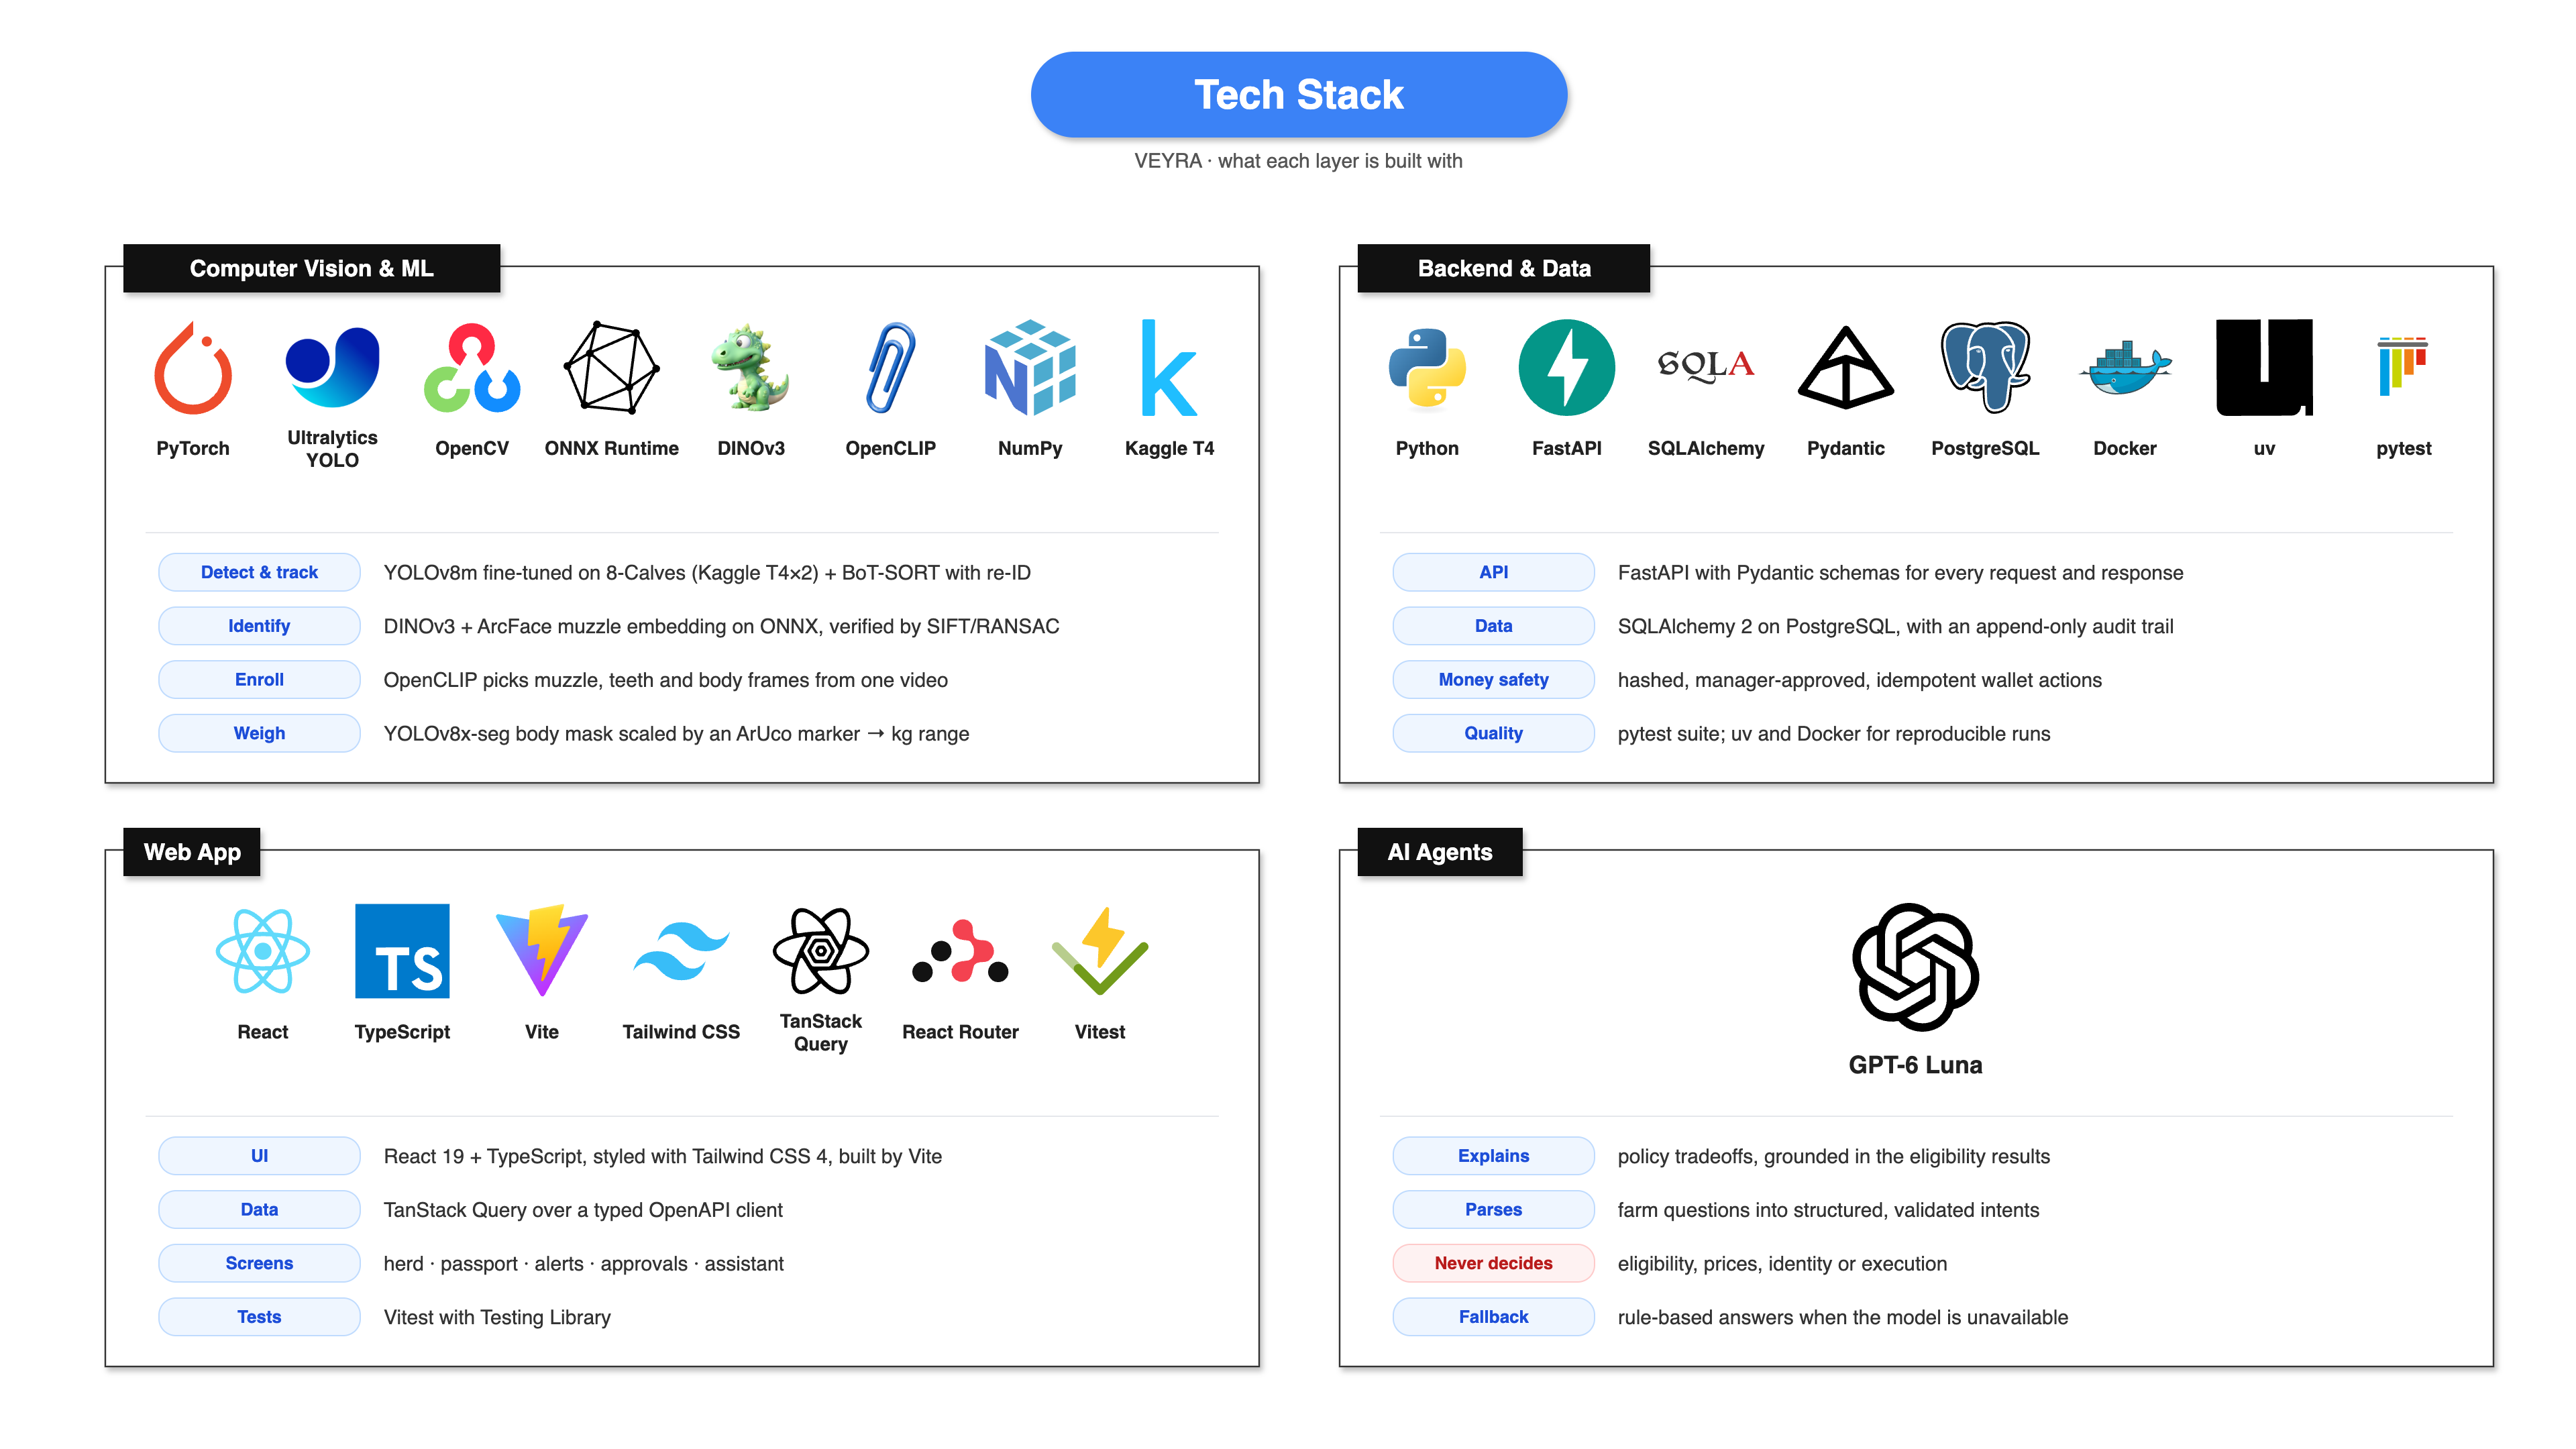
\includegraphics[width=\textwidth]{figures/tech_stack.png}
\caption{Technology stack by layer.}
\label{fig:stack}
\end{figure}

\begin{figure}[H]
\centering
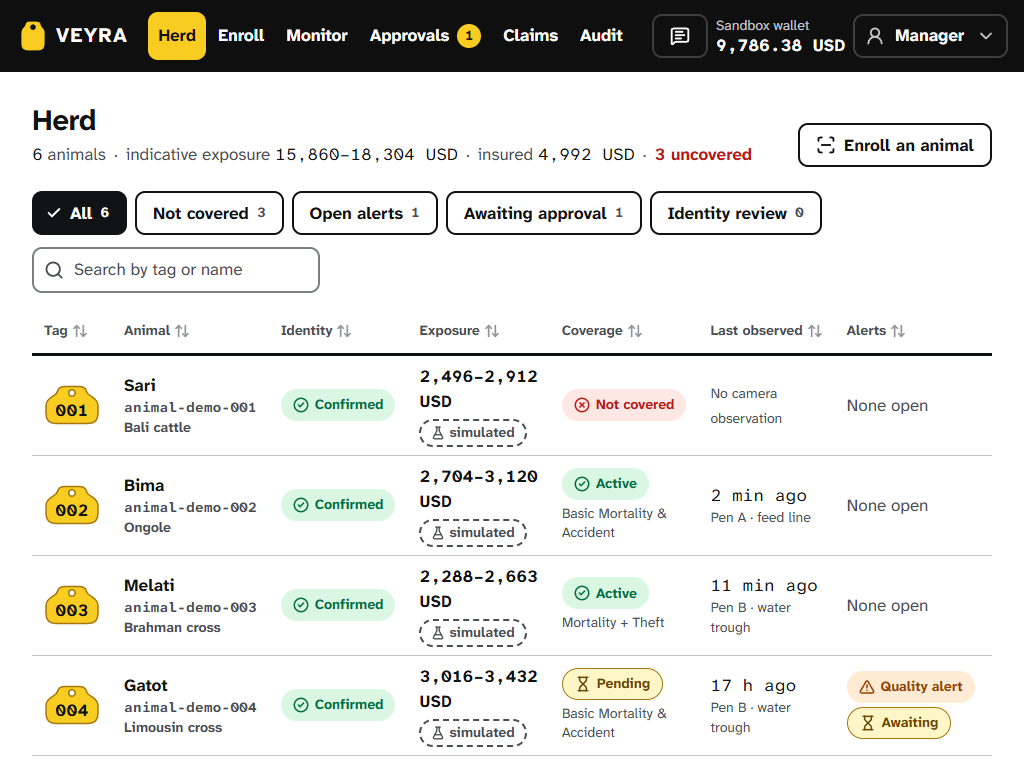
\includegraphics[width=0.85\textwidth]{figures/app_herd_1024.png}
\caption{Herd overview: every row is one passport with its indicative exposure, coverage, last camera sighting, and open alerts.}
\end{figure}

\begin{figure}[H]
\centering
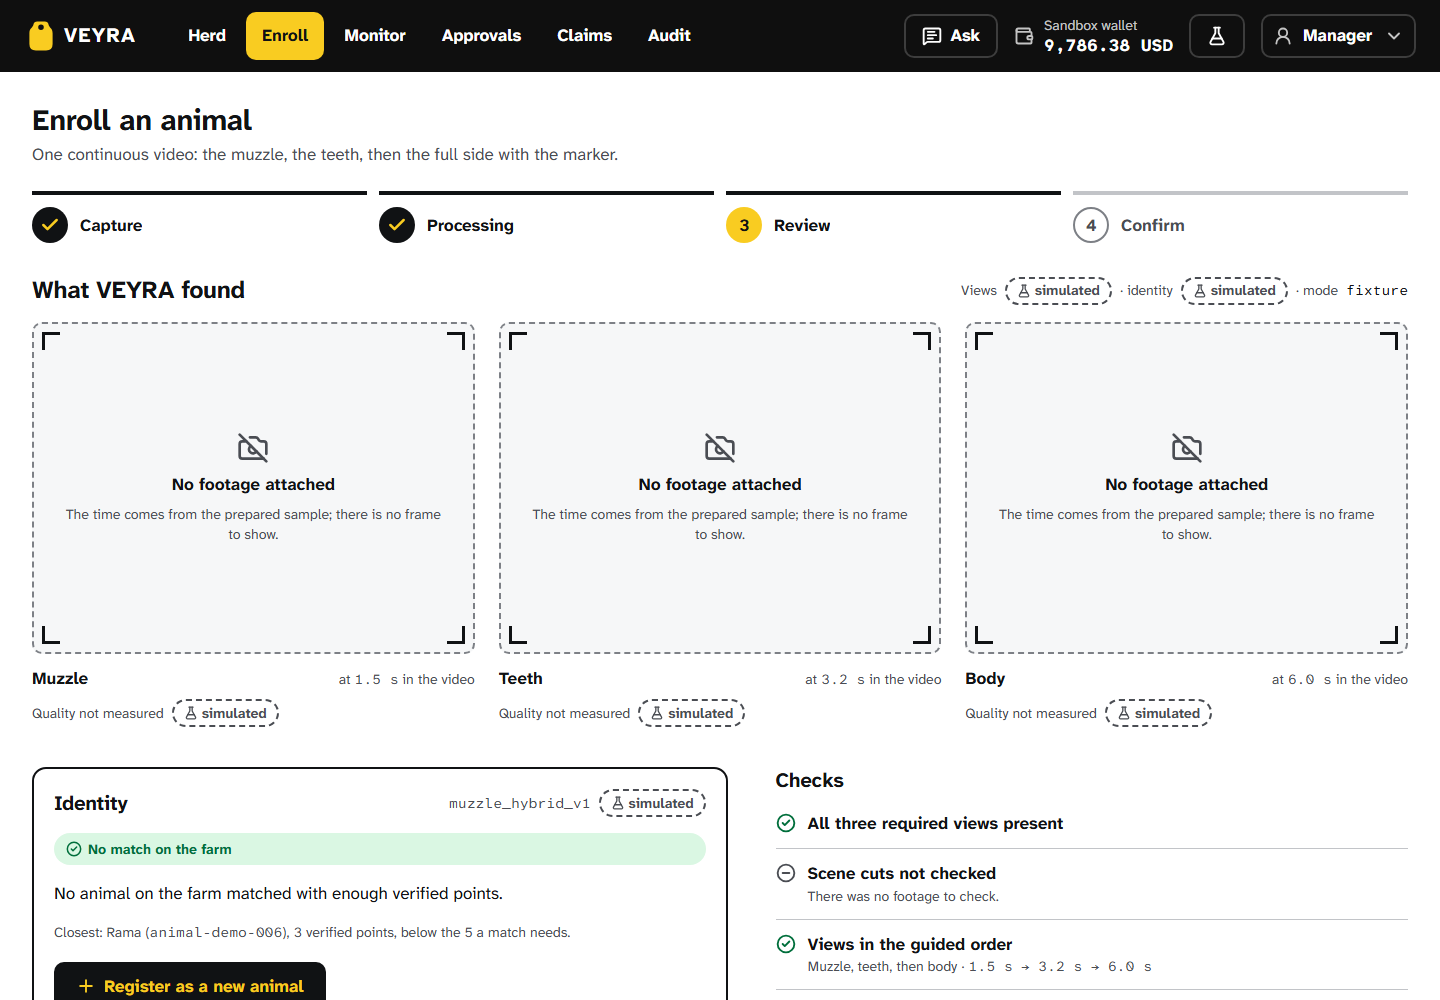
\includegraphics[width=0.95\textwidth]{figures/app_enroll_review.png}
\caption{Enrollment review: the registered views, the quality checks, and the identity outcome presented for human confirmation.}
\end{figure}

\begin{figure}[H]
\centering
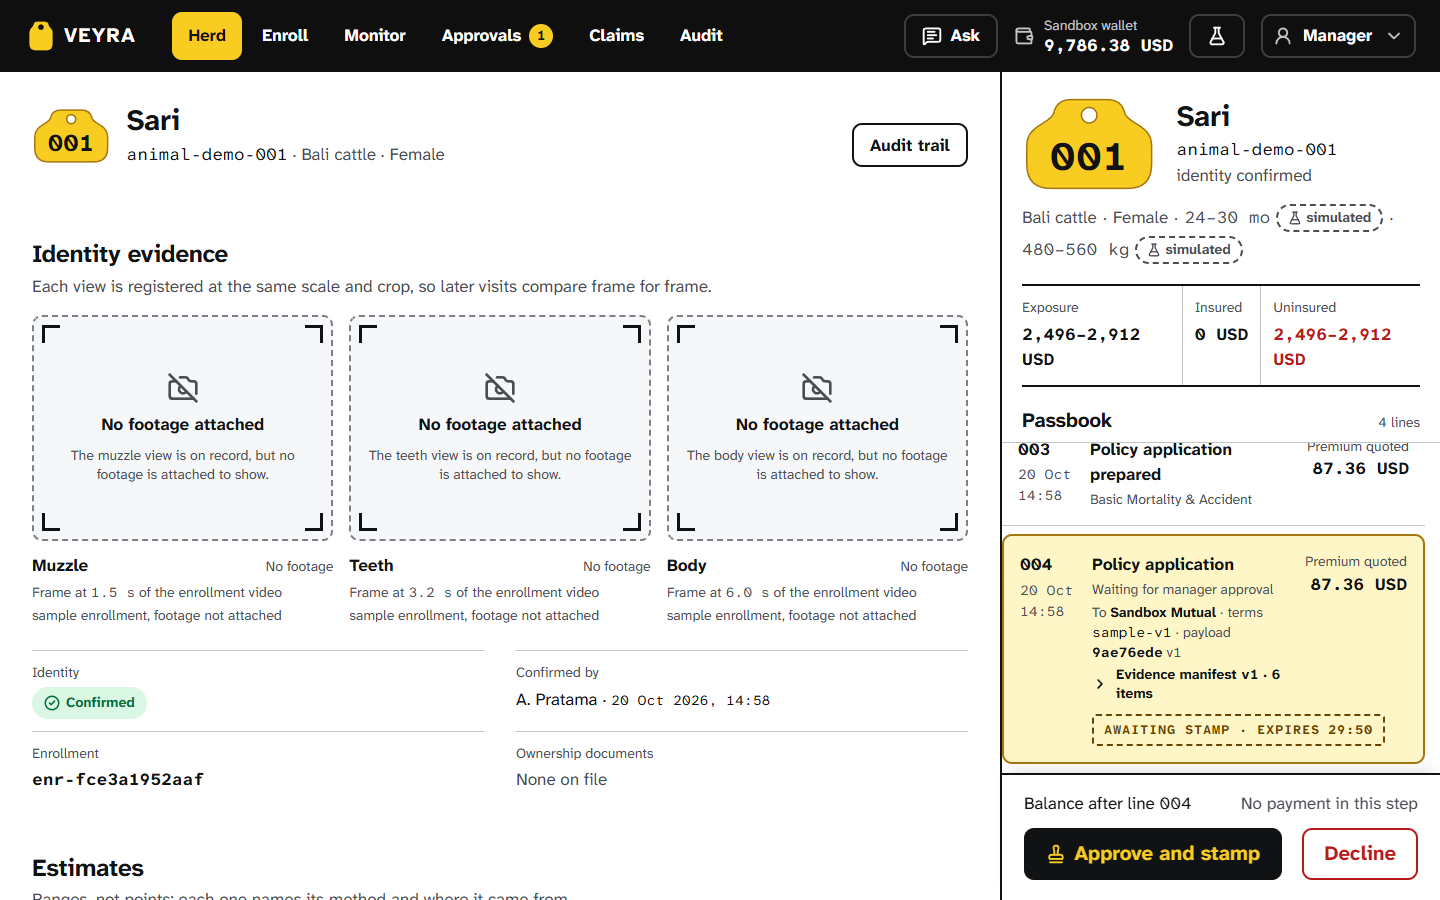
\includegraphics[width=0.95\textwidth]{figures/app_passport_desktop.png}
\caption{Digital Livestock Passport: identity evidence, estimates with their provenance, and the passbook of insurance actions.}
\end{figure}

\begin{figure}[H]
\centering
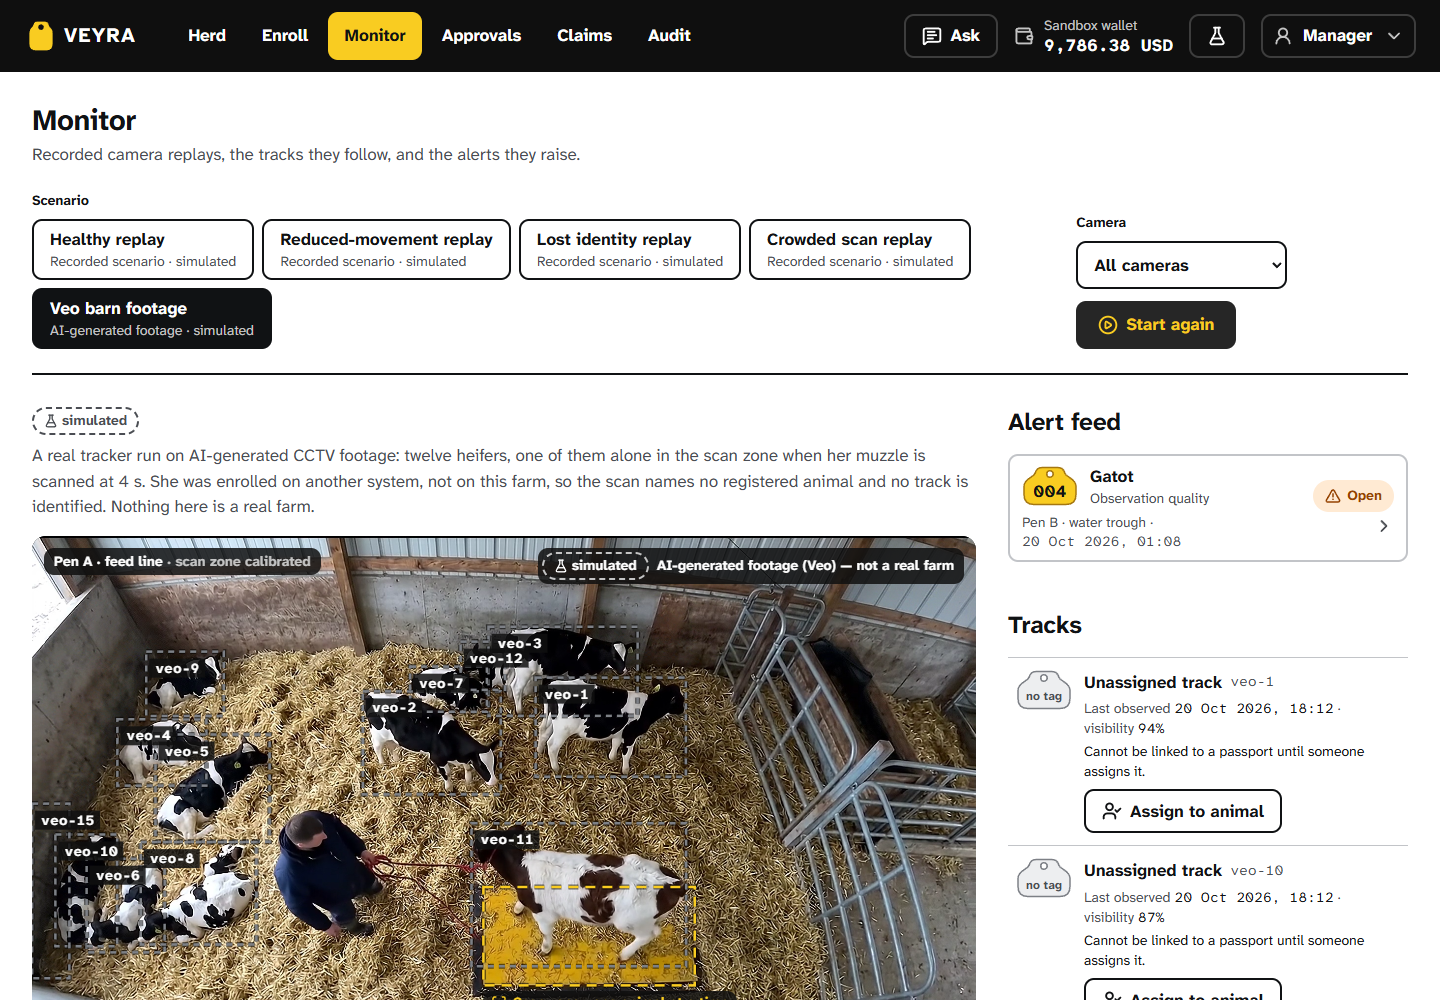
\includegraphics[width=0.95\textwidth]{figures/app_monitor_veo.png}
\caption{Monitor: the barn camera with tracks, the scan zone, the alert feed, and the pen map.}
\end{figure}

\begin{figure}[H]
\centering
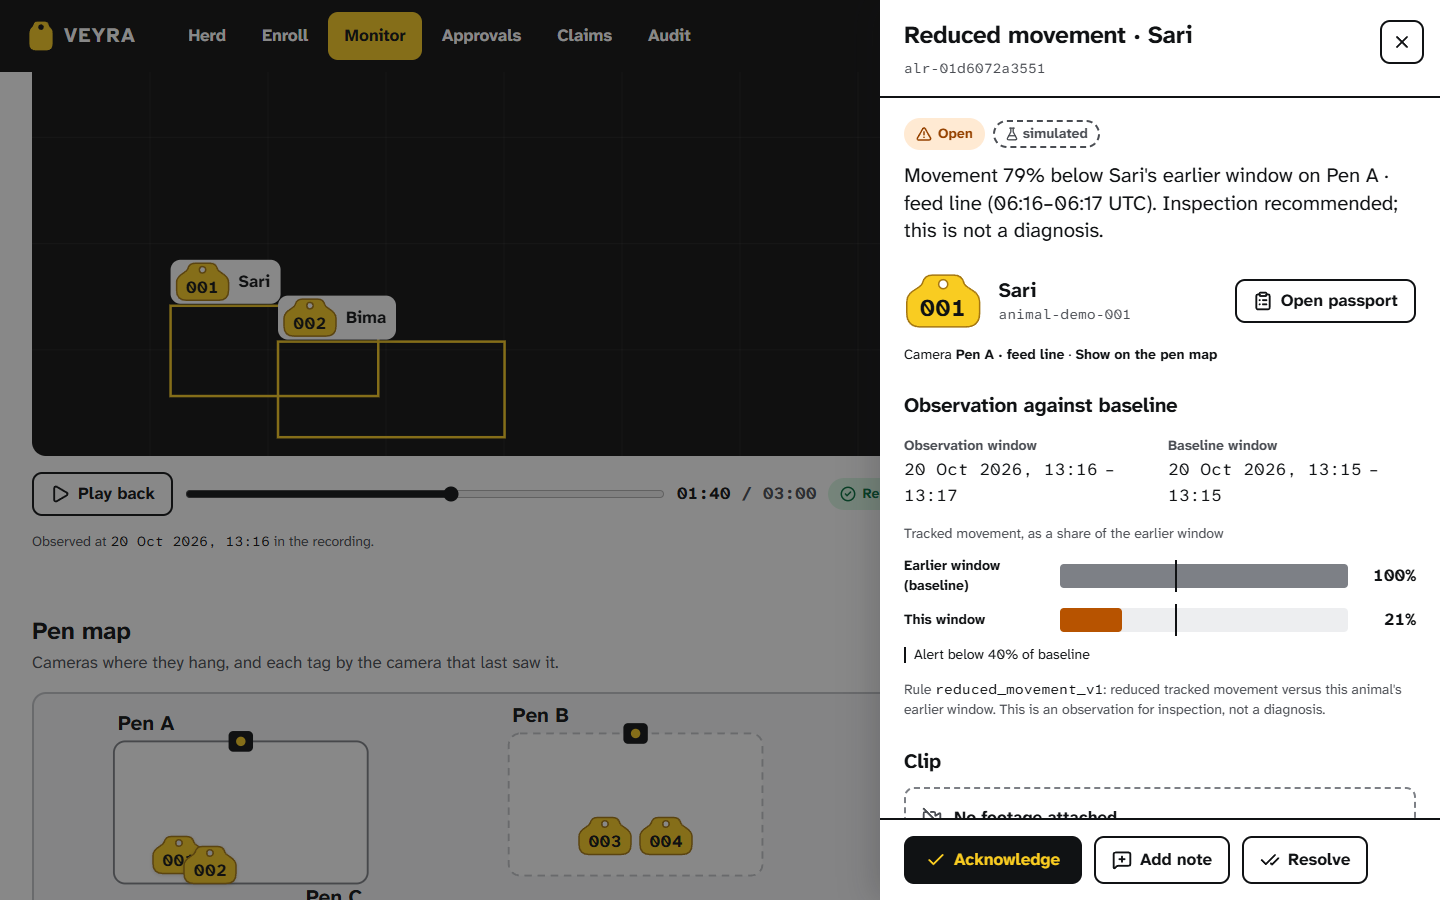
\includegraphics[width=0.95\textwidth]{figures/app_alert_drawer.png}
\caption{Reduced-movement alert: the observation window against the animal's own baseline, the measured drop, and a recommended inspection.}
\end{figure}

\begin{figure}[H]
\centering
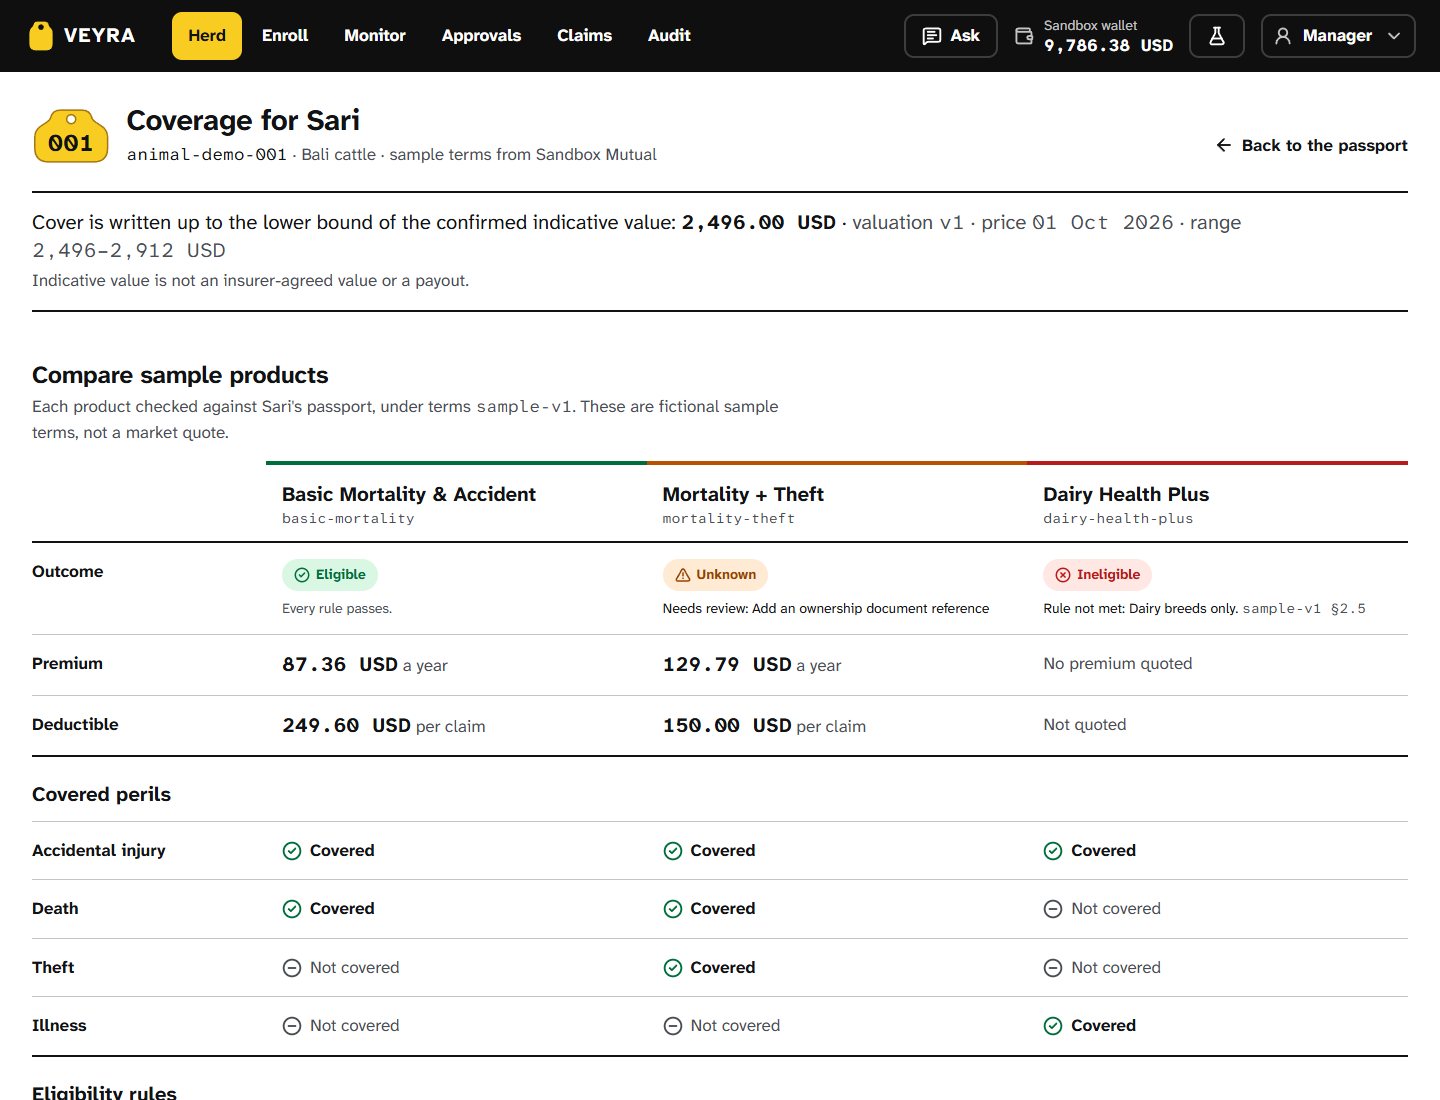
\includegraphics[width=0.95\textwidth]{figures/app_insurance_desktop.png}
\caption{Coverage comparison: eligibility per product with the rule and terms reference behind each outcome, premiums, deductibles, and exclusions.}
\end{figure}

\begin{figure}[H]
\centering
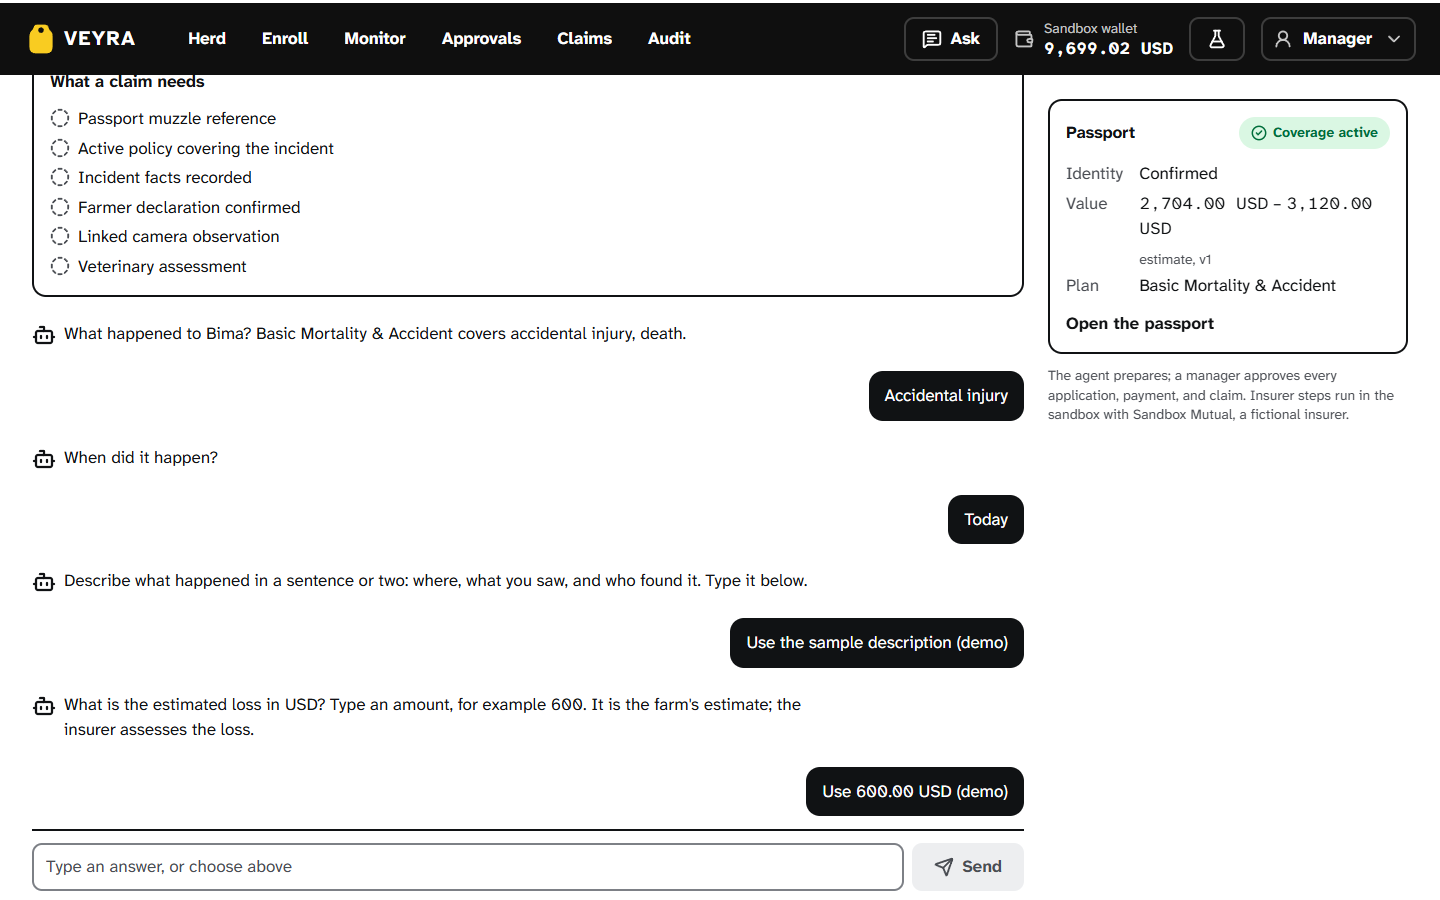
\includegraphics[width=0.95\textwidth]{figures/app_agent_desktop.png}
\caption{The in-app VEYRA agent guiding a claim with typed, record-backed cards.}
\end{figure}

\begin{figure}[H]
\centering
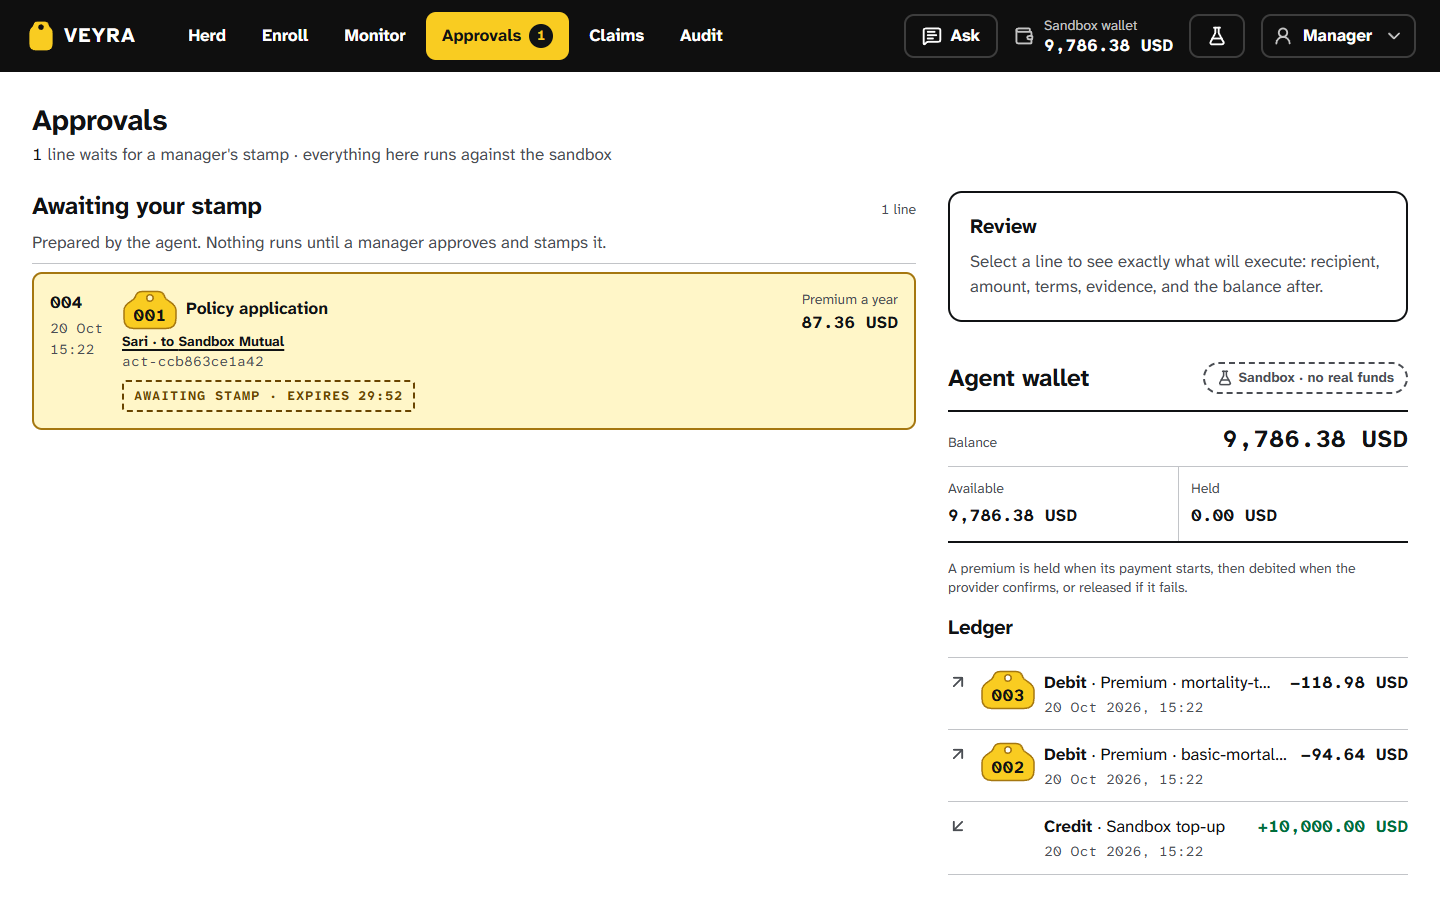
\includegraphics[width=0.95\textwidth]{figures/app_approvals_desktop.png}
\caption{Approvals and the agent wallet: a prepared action awaits the manager's stamp, with the sandbox balance, holds, and ledger.}
\end{figure}

\begin{figure}[H]
\centering
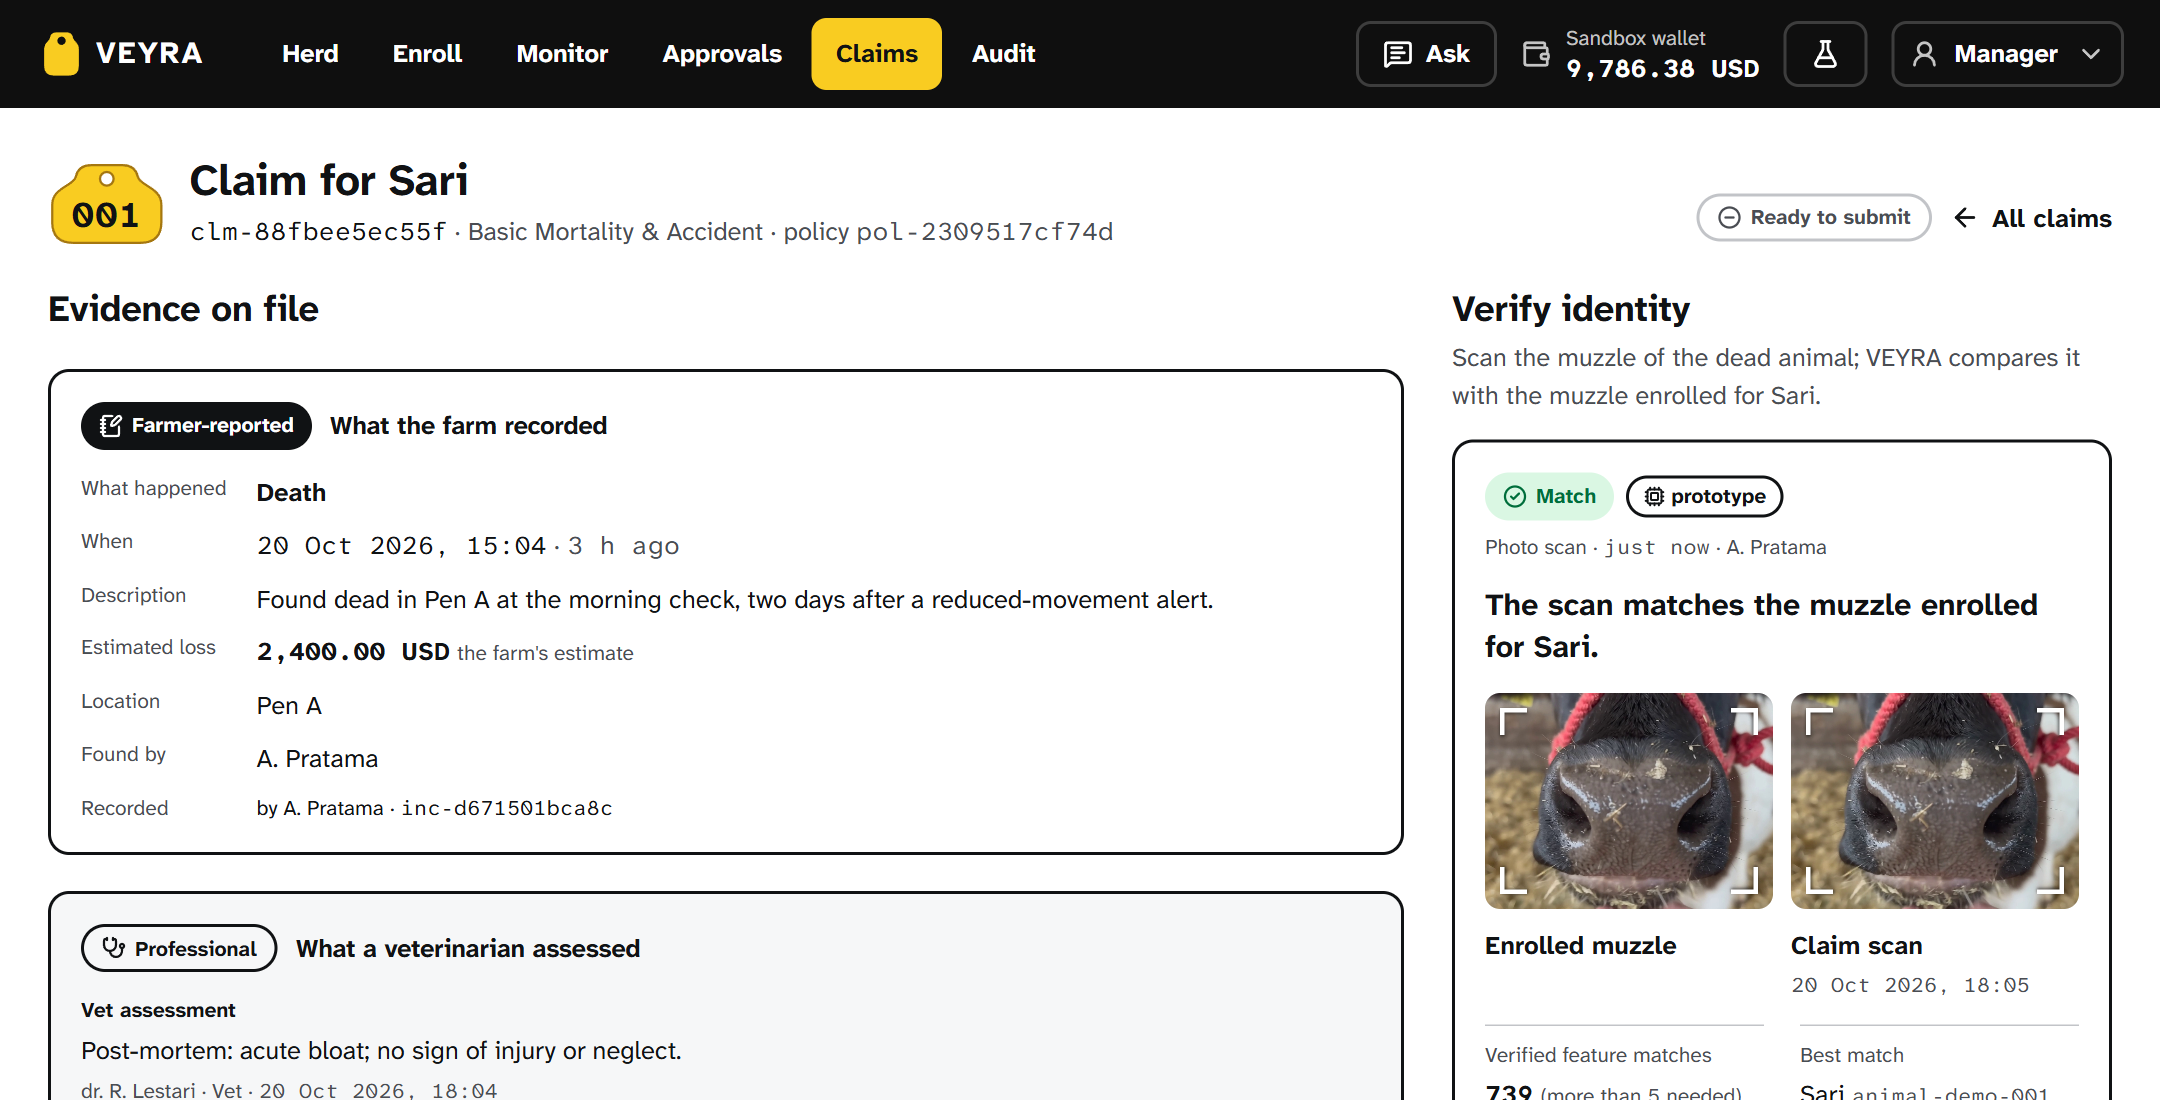
\includegraphics[width=0.95\textwidth]{figures/app_claim_identity_match.png}
\caption{Claim-time identity check: a fresh muzzle scan matched against the claimed animal and every other confirmed animal.}
\end{figure}

\begin{figure}[H]
\centering
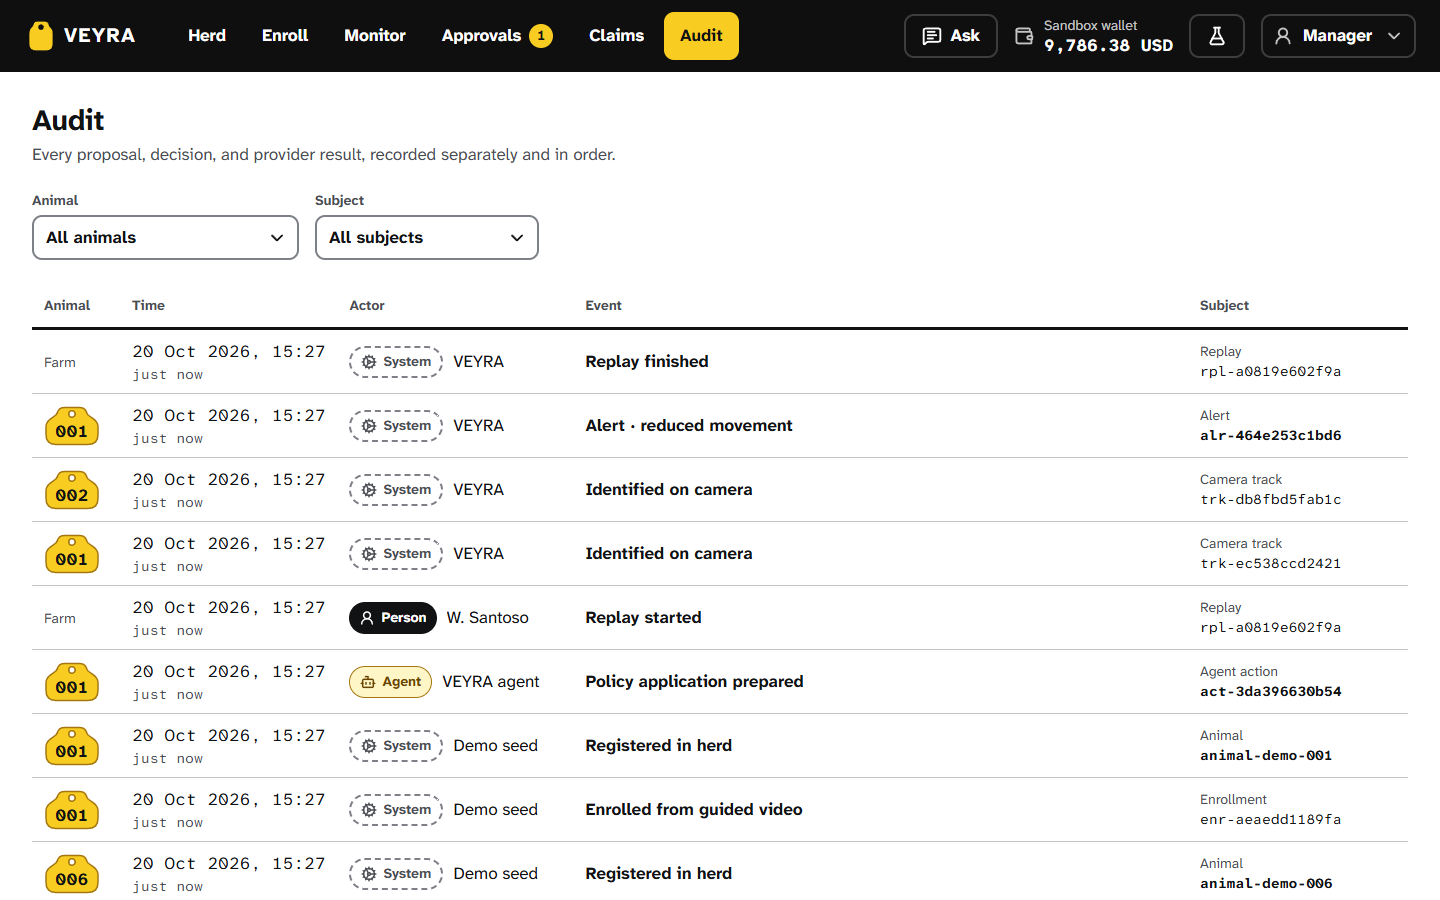
\includegraphics[width=0.95\textwidth]{figures/app_audit_desktop.png}
\caption{Audit trail: agent proposals, manager decisions, and provider results as separate events, each tied to one animal.}
\end{figure}

\section{Appendix B: Product Links}

\noindent GitHub repository: \url{https://github.com/ShibainuID/Veyra}

\end{document}
